
% Cal Poly Thesis
% 
% based on UC Thesis format
%
% modified by Mark Barry 2/07.
%




\documentclass[12pt]{ucthesis}

\newif\ifpdf
\ifx\pdfoutput\undefined
    \pdffalse % we are not running PDFLaTeX
\else
\pdfoutput=1 % we are running PDFLaTeX
\pdftrue \fi

\usepackage{url}
\ifpdf

    \usepackage[pdftex]{graphicx}
    % Update title and author below...
    \usepackage[pdftex,plainpages=false,breaklinks=true,colorlinks=true,urlcolor=blue,citecolor=blue,%
                                       linkcolor=blue,bookmarks=true,bookmarksopen=true,%
                                       bookmarksopenlevel=3,pdfstartview=FitV,
                                       pdfauthor={Gregory Flanagan},
                                       pdftitle={Conceptual Requirement Validation for Architecture Design Systems},
                                       pdfkeywords={thesis, masters, cal poly}
                                       ]{hyperref}
    %Options with pdfstartview are FitV, FitB and FitH
    \pdfcompresslevel=1

\else
    \usepackage{graphicx}
\fi

\usepackage{amssymb}
\usepackage{amsmath}
\usepackage[letterpaper]{geometry}
\usepackage[overload]{textcase}
\usepackage{subfig}
\usepackage{float}
\usepackage{amssymb}

\bibliographystyle{abbrv}

\setlength{\parindent}{0.25in} \setlength{\parskip}{6pt}

\geometry{verbose,nohead,tmargin=1.25in,bmargin=1in,lmargin=1.5in,rmargin=1.3in}

\setcounter{tocdepth}{2}
\graphicspath{{fig/}}


% Different font in captions (single-spaced, bold) ------------
\newcommand{\captionfonts}{\small\bf\ssp}

\makeatletter  % Allow the use of @ in command names
\long\def\@makecaption#1#2{%
  \vskip\abovecaptionskip
  \sbox\@tempboxa{{\captionfonts #1: #2}}%
  \ifdim \wd\@tempboxa >\hsize
    {\captionfonts #1: #2\par}
  \else
    \hbox to\hsize{\hfil\box\@tempboxa\hfil}%
  \fi
  \vskip\belowcaptionskip}
\makeatother   % Cancel the effect of \makeatletter
% ---------------------------------------




\begin{document}

% Declarations for Front Matter

% Update fields below!
\title{Conceptual Requirement Validation for Architecture Design Systems}
\author{Gregory Flanagan}
\degreemonth{September} \degreeyear{2010} \degree{Master of Science}
\defensemonth{September} \defenseyear{2010}
\numberofmembers{3} \chair{Franz Kurfess, Ph.D.} \othermemberA{Mehul Bhatt, Ph.D.} \othermemberB{John Seng, Ph.D.} \field{Computer Science} \campus{San Luis Obispo}
\copyrightyears{seven}



\maketitle

\begin{frontmatter}

% Custom made for Cal Poly (by Mark Barry, modified by Andrew Tsui).
\copyrightpage

% Custom made for Cal Poly (by Andrew Tsui).
\committeemembershippage

\begin{abstract}
 



\end{abstract}

%\begin{acknowledgements}

%   Thank you...

%\end{acknowledgements}


\tableofcontents


\listoftables

\listoffigures

\end{frontmatter}

\pagestyle{plain}




\renewcommand{\baselinestretch}{1.66}


% ------------- Main chapters here --------------------





\chapter{Introduction}
\label{intro}


This is the introduction.



\chapter{Preliminaries}
\label{preliminaries}

\section{Qualitative Spatial Representation and Reasoning}
\subsection{Applications of Spatial Reasoning}
\subsubsection{Architectural Design}
\subsubsection{Geographic Information Systems}
\subsubsection{Robotics}
\section{Constraint Logic Programming}


\chapter{Previous Work}
\label{previous-work}
\section{Design Support Systems}
\subsection{SEEDS}
The SEEDS project, described in \cite{FlemmingIKM94}, proposed a architectural design platform for capturing and representing functional (i.e. spatial requirements) and structural (geometric) design knowledge. The aim of which is to support the architectural design process by providing design knowledge during the initial design phase of a building. Within the SEEDS project, design knowledge is partitioned into two categories: design units, and functional units. Design units represent spatial and physical elements of a building, while functional units represent requirement that constrain design units
based on shape, size, placement, etc.. Additionally, SEEDS pioneered the idea that architectural design knowledge, specifically design requirements, could be represented as constraints to automatically generate layouts.



\section{AI in Design}
\subsection{Intelligence Virtual Environments}
Caldern \cite{CalderónCLP06} built upon the ideas in \cite{FlemmingIKM94} for representing design knowledge, to develop an Intelligent Virtual Environment that solves spatial configuration problems based on spatial design knowledge. Additionally, the tool added non-geometric semantics (i.e. environmental, lighting) for functional units to demonstrate that their approach could be extended to non-geometric design knowledge.

Caldern argued that spatial knowledge By representing design knowledge as constraints, the tool was able to use constraint logic programming to solve spatial configuration problems. In general, constraint are classified as: topological, local, and global. Topological constraints describe the topological characteristics of the environment, such as a regions where a lighting is less then 300 lux. Local constraints describe the attributes of a
single object and how it interacts with topological characteristics. In general these characteristics are in the form of, a desk should be at least 4 meters from a ventilation duct, or an object should be within an area that has more then 300 lux of light. Global constraints express design requirements for a group of objects.  

Axling \cite{AxlingEURO96} and Codognet \cite{CodognetDMS99} proposed the use constraint  logic programming in Virtual Environments for intelligent object behavior. Their approaches focuses on the behavior of single objects without taking into consideration behavior of a set of object or how objects constrained by the specific environment. 

\subsection{V-SIMSPLACE}
\cite{LertlakkhanakulIBPSA06} describes a platform that 'embodies spatial context-aware information' so that users can visualize an architectural design before it is deployed. The aim of the tool is to simulate a users experience in a Smart Home environment, in order to study the interactions of the user within his/her environment. The crux of the system is that behavioral semantics of a Smart Home are integrated into the building design knowledge so that the interactions a user has within the Virtual Environment will closely mimic the real world.

Unlike \cite{CalderónCLP06}, V-PLACESIMS does not attempt to capture design requirements or reason about the consistency of an environment. Rather, it's focus is providing a platform for users to interact with a Smart Home environment to discover the behaviors and interactions that take place.

\subsection{Intelligence for Ambient Design}
Bhatt proposed a system in \cite{BhattDH09} that provides validation for the satisfiability of functional requirements, which are grounded to a qualitative spatial calculi, within the Ambient Environment domain. The system accomplishes this by modeling the functional requirements as constrains in an ontology and uses an ontology reasoner to discover if a model is realizable for a design, i.e. no models will be found if on or more functional constraints are not satisfied. 

\subsection{Decision Support for Virtual Environment}
\cite{Nomura92} used a Decision Support System to validate the design configuration. The system was used more as a diagnostic system, rather then providing feedback on how to reconfigure the environment. Note: I have not read \cite{Nomura92} because I haven't been able to track it down. Therefore my description here is based on the related works section of \cite{CalderónCLP06}.



\chapter{DSpace Reasoner}
The DSpace Reasoner is a prototype tool for validating conceptual design requirements against CAAD based architectural design plans. Conceptual design requirements here refer to requirements as they pertain to the functional and experiential aspects of the design from a semantic and qualitative perspective. For example, architects commonly describe aspects of a design in a qualitative fashion, such as a design being private, accessible, or continuous. These architectural aspects emerge from the spatial structures / arrangements of the building form and are experienced in the building. 

The goal of the DSpace reasoner is to build a computational framework to represent and reason about conceptual design requirements to validate conceptual design requirement to the real world, CAAD based architectural plans.     


\section{Design Problem}
State-of-the-art CAAD tools represent the physical and structural aspects of an architectural design in a manner that is both accurate and precise. This type of representation captures the design, in terms of the spatial features, spatial dimensions of architectural entities, placement of entities within the building, at a low-level of granularity that is needed in the actual construction of the building, and allows for reasoning about the physical, structural and mechanical aspects of a design with regard to the precise geometric representation; such as the placement of a door in a wall or the mechanics of a window swinging open and closed. TODO: talk about x,y,z coordinates of real space, quantitative representation.

However, this type of representation scheme does not incorporation the qualitative and functional features of the design. For example, a structural design requirement that addresses air circulation stipulates that a doorway and window should face directly towards each other. For a traditional CAAD based system, reasoning about such a requirement is not possible because it pertains to qualitative spatial design features and functional attributes that go beyond the purely geometric representation of the design, i.e., in this case the qualitative spatial relationship between a window and doorway.

This representation allows an architect to validate a work-in-progress design from a conceptual and qualitative perspective against the physical and precise real world geometrical representation of the design \cite{Bhatt}.

 The crux of this is that it bridges the gap between the quantified geometries and the functional / qualitative requirements of the design, thus allowing the reasoner to validate a high level requirement against its precise geometric representation. 

to do this dspace need to:
 - representation of design
 	- spatial abstraction / multiple perspectives
 	- artefacts
 - design requirements - define / identify
 	- define architectural qualities
 		- perceptual
 		- intrinsic / geometric
 	- define architectural concepts
	- spatial interpretation / explicit characterization
 - qualitative spatial reasoning
 	- topological 
 	- orientation
 		- intrinsic vs extrinsic
 	- distance

\section{Multi-Hierarchy}
The design multi-hierarchy developed in this section is built on the mapping of the design problem into a design space, a quality space, and a quantity space. At the highest level, the design space involves the architectural design semantics (architectural concepts) and qualities (qualitative spatial attributes found in architecture) that emerge in architecture. At the lowest level, the quantitative space involves the precise geometries of the architectural structures found in the design. The qualitative space mediates between the abstractions of the design layer and the concreteness of the quantitative later using qualitative spatial representation and reasoning.
 
\begin{figure}[H]
\centering

\includegraphics[width=140mm]{hierarchy2}
\caption{Design Space Multi-Hierarchy}
\label{hierarchy}
\end{figure}

Figure \ref{hierarchy} shows the design multi-hierarchy used in the DSpace reasoner. Conceptual design requirements are built from the architectural concepts and qualitative spatial attributes found in architecture (QSA) of the hightest level of the multi-hierarchy. Within the multi-hierarchy, architectural concepts are built using QSA, but are not limited to only these, spatial relationships of orientation, topology, and distance can be used, as well as other geometric primitives such as area, angle, and length measurements. QSA are defined by the qualitative spatial relationships of orientation, topology, and distance. These qualitative spatial relationships emerge from the quantitative, physical, and artefactual geometries of the the design. TBD: physical structures define the way the architecture is experiences and influences the functional / performance of the design from a conceptual design perspective.

\section{DSpace: Design and Implementation}
\begin{figure}[H]
\centering

\includegraphics[width=130mm]{design}
\caption{DSpace Design}
\label{dspace design}
\end{figure}


\subsection{Factbase}
Prolog facts make up a factbase that stores a table of architectural entities with their architectural types (e.g., wall, door, window, desk, etc.). Each architectural entity in the design has a single entry in the factbase. The factbase is instantiated automatically during the import process from a CAAD based representation. This factbase will be used throughout the DSpace reasoner to  verify an entity exists in the design and links it to its architectural type. The following Prolog code shows two instantiated facts (predicates) for a doorway, and a window. 
\begin{verbatim}
   architectural_entity(door1, dSDoor).
   architectural_entity(wall4, dsWindow).
\end{verbatim}


\chapter{Design Representation and Spatial Reasoning}
This chapter presents the architectural design representation and spatial reasoning framework of the DSpace reasoner. It examines how architectural designs are modeled in a multiple perspective representation structure, and how architectural designs are reasoned about using qualitative spatial representation and reasoning techniques. The DSpace framework is written in the declarative programming semantics of Constraint Logic Programming (CLP) using Prolog, CLP over the Reals (CLP($\mathbb{R}$)), and Constraint Handling Rules (CHR).  

The chapter is organized into two sections. The first section looks at how architectural design are represented in DSpace and how this representation model is implemented in the DSpace CLP framework. The second section looks at the DSpace spatial reasoner and how it is implemented as a series of spatial constraint solvers in the DSpace CLP framework.

\section{Design Representation in DSpace}
DSpace represents multiple aspects of a design. It represents the physical features as they pertain to the design's geometric structures, and the functional features as they pertain to the design's non-physical artefactual extensions. This design representation goes beyond what is represented in CAAD programs and allows for reasoning over the design

In DSpace an architectural design is modeled in a multiple perspective representation structure that incorporate aspects of the design that are quantitative, functional, and abstract. This design representation goes beyond what is represented in CAAD programs by incorporating design features that are not based on the design's quantitative design representation. It includes functional aspects of the design that pertain to the performance and functional features of the design, as well as abstract spatial aspects that pertain to the qualitative feature space of the design. The objective of this representation structure is to provide the DSpace reasoner with mechanisms that connect an expert's high level design conceptualizations to the low level geometric quantities of a CAAD based system.   

\begin{figure}[H]
\centering

\includegraphics[width=90mm]{multi-persepective}
\caption{Multiple Perspective Structure}
\label{mutli-perspective}
\end{figure}

Within the CLP framework of DSpace, the multiple perspective model is implemented as a set of Prolog rules. These rules bind architectural entities, via their DSpace identifier (\emph{dsID}), to their multiple perspective representations. Combining these rules for each entity creates a rulebase that stores the multiple perspective representation in the DSpace CLP framework. This rulebase can be queried to retrieve a specific geometry given a \emph{dsID}. Figure \ref{clp-design} shows the implementation design for the multiple representation structure in the DSpace CLP framework. Notice that all rules are accessed via the factbase, which stores \emph{dsID}'s and ensures that an entity exists before the rulebase is queried. Additionally, all representations are defined over the same set of spatial primitives. This uniformity will be an important aspect of the spatial reasoner in the next section. 

\begin{figure}[H]
\centering
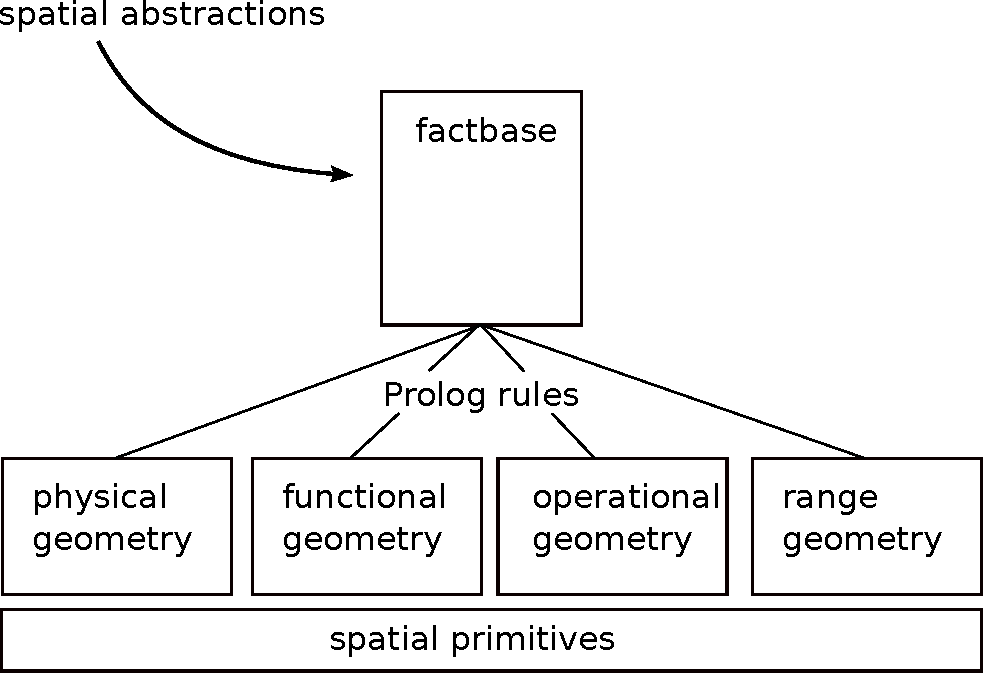
\includegraphics[width=90mm]{clp-design}
\caption{Representation in CLP}
\label{clp-design}
\end{figure}

The remainder of this section looks at the three design representation perspective individually: quantitative, functional, abstract.

\subsection{Quantitative Perspective}
The quantitative representation of the design models the structural form of the design in terms of its precise physical geometric features (i.e., layout, shape, location). Architectural entities, such as walls, windows, doorways, columns, and rooms, are represented as geometric primitives of polygons, lines and points that correspond to the physical dimensions (length, width, shape) of the entities. The quantitative model of DSpace represents the design perspective that is similar to CAAD programs.

Within the DSpace CLP framework, the quantitative geometry is defined by geometric primitives of polygons, lines, and points. These primitives are defined by Prolog rules that consume quantitative point data and return an instantiated spatial primitive. The following Prolog rules shows an example of a quantitative rule definition for an entity with \emph{dsID window445}. This rule will be stored in the DSpace rulebase. 
\begin{verbatim}
    quantitative_geometry(window445, Geometry) :-
            spatial_primitive(Geometry, [(1,1),(3,5),(4,5),(2,2)]).
\end{verbatim}
Given an entity and its \emph{dsID}, a query to the DSpace rulebase will return an instantiated variable with the entity's quantitative geometry.  
If the following query is made, the quantitative geometry of \emph{window445} will be instantiated in the \emph{Geometry} variable.
\begin{verbatim}
    quantitative_geometry(window445, Geometry).
\end{verbatim} 


\subsection{Functional Perspective}
Spatial artefacts are non-physical, spatial extensions of architectural entities that pertain to a specific functional quality of an entity. Artefactual extensions do not have a physical manifestation; however, they are an important part of the design representation because they affect the functionality and performance of the design. There are three types of spatial artefacts identified by Bhatt\cite{Bhatt} that are represented in DSpace: \emph{operational space}, \emph{functional space}, and \emph{range space}.

\begin{figure}[H]
 \centering
 \subfloat[operational space]{\label{operational-space}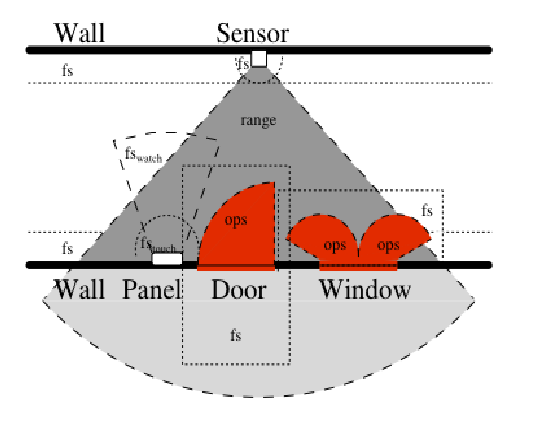
\includegraphics[width=43mm]{operational-space}}
 \hspace{7 mm}
 \subfloat[functional space]{\label{functional-space}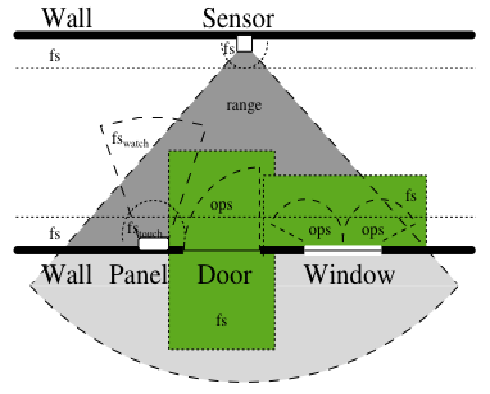
\includegraphics[width=40mm]{functional-space}}
  \hspace{7 mm}
 \subfloat[range space]{\label{range-space}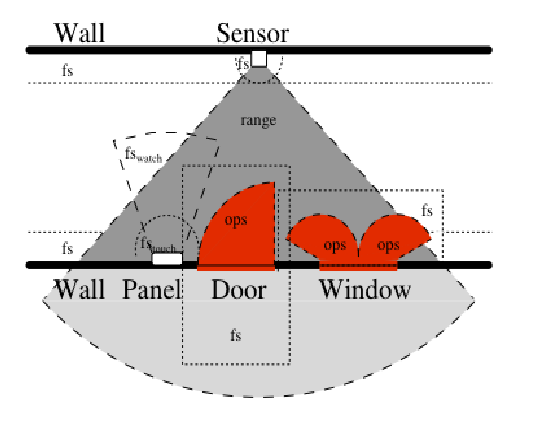
\includegraphics[width=43mm]{operational-space}}
 \caption{Artefactual Extensions}
\label{artefactual-extensions}
\end{figure}

The operational space encompasses the region of space required by an object to preform its function. For example, the operational space of a door is the area in which a door can occupy during its operation, opening and closing (see figure \ref{operational-space}). This space is dynamic in the sense that it represents the configurable space of the physical doorway. 

The functional space encompasses the region of space that is required for an object to function itself or the space for a person to operate an object. For example, the functional space of a doorway is the total area needed for a person to operate, open and close, as well as any additional space need to navigate entirely through the doorway (see figure \ref{functional-space}). 

The range space pertains to a region of space that encompass the range of a sensor (i.e., camera, motion sensor). For example, the range space of a camera is defined by its depth of field and angle of view. It represents the total space that is under surveillance of the camera (see figure \ref{range-space}).

\begin{figure}[H]
\centering
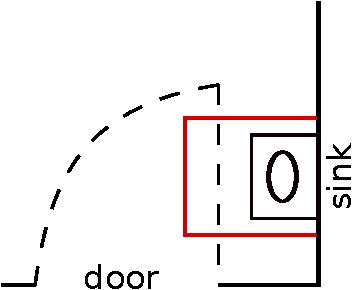
\includegraphics[width=50mm]{door-sink}
\caption{Operational Space Interference}
\label{door-sink}
\end{figure}

Artefactual extensions directly affect how well a design functions. For example, a sink in a bathroom has a functional space, the space a person occupies while washing his/her hands at the sink. If this space interferes with (i.e., topologically overlapping) the functional and/or physical space of a doorway, this will cause a circulation problem when both the doorway and sink are simultaneously being operated, i.e., a collision between the person washing his/her hands and the doorway itself or the person operating the doorway. In this example, the functional aspects of the bathrooms design with regard to the mitigation of circulation problems is directly influenced by the spatial configuration of the non-physical artefactual extensions of the design. 

Within the DSpace CLP framework, artefactual geometries are defined using the same spatial primitives as the quantitative geometries. The main difference between the two is that there are multiple rules, one for each artefactual type: functional, operational, and range. An entity may have zero or more artefactual geometries. For example, a doorway in general has a functional and operational representation but does not have one for range representation, while a column has no artefactual representations. The following Prolog rules show and example of a rule definition for the functional and operational representations for a doorway with \emph{dsID} of \emph{door55}. 
\begin{verbatim}      
    functional_geometry(door55, Geometry) :-
            spatial_primitive(Geometry, polygon(PtList)).
           
    operational_geometry(door55, Geometry) :-
            spatial_primitive(Geometry, polygon(PtList)).
\end{verbatim}
Given an entity and its dsID, a query to the DSpace rulebase will return an instantiated variable with the entity’s artefactual geometry. Which geometry is returned is based on the rule that is queried. If the following functional representation query is made, the functional geometry of \emph{door55} will be instantiated in the FuncGeometry variable.
\begin{verbatim}
   functional_geometry(door55, FuncGeometry).
\end{verbatim}


\subsection{Abstract Perspective}
In DSpace architectural entities have spatially abstracted representations. This allows DSpace to reason about a design from a qualitative level of abstraction with regards to its spatial characteristics of topology, orientation and distance. This type of qualitative spatial reasoning reasons over the abstract feature space of the design using abstract spatial objects of points, directed points, and convex hulls. 

Architectural entities are not directly modeled as abstract spatial objects, as they are in the other representations. Abstract spatial objects are generated by transformation rules that abstract the quantitative geometries of the architectural entities. The process of spatially abstracting an architectural entity depends on the spatial characteristics of the entity's structural form, and an interpretation of the intrinsic nature of an entity within an architectural / design context. For example, the abstracted representation of a doorway as a directed point is defined not only by its physical form but also by the interpretation of the doorway's intrinsic direction. 

Within the DSpace CLP framework, Prolog rules transform quantitative geometries into spatially abstracted objects (i.e., spatial abstraction). Spatially abstracting an architectural entity depends on the entity type, the spatial abstraction type (point, directed point, or convex hull) and sometimes a contextual identifier (direction of a doorway into or out of a specific room). Given these dependencies, spatially abstraction rules geometrically transform the quantitative geometries into abstract spatial objects. 

Unlike the quantitative and functional representations, the abstract representation is not stored in the rulebase. Rather, spatial abstraction rules function over the quantitative and functional rulebase. For example, the spatial abstraction rule for a doorway into a point abstraction requires the point abstraction rule to query the quantitative rulebase to retrieve the doorways quantitative geometry. The following spatial abstraction rule is for a doorway point abstraction. Note that the rule is based on the interpretation of a doorway point abstraction as the centroid of its quantitative geometry (see Appendix A.1).   
\begin{verbatim}
    point_abstraction(door55, PtAbs) :-
            quantitative_geometry(door55, Quant),
            centroid(Quant, PtAbs).
\end{verbatim}
Given an entity and its dsID, a query to the DSpace spatial abstraction rule will return an instantiated variable with the entity's spatially abstracted geometry. If the following query to the point abstraction rule is made for a doorway with \emph{dsID} of \emph{door55}, then the point abstraction geometry of \emph{door55} will be instantiated in the PtAbs variable.
\begin{verbatim}
    point_abstraction(door55, PtAbs).
\end{verbatim}


\section{Spatial Reasoning in DSpace}
In DSpace qualitative spatial reasoning serves as a link between the high level conceptual design space and the low level quantitative geometric space. It uses formal qualitative spatial calculi for topological (Region Connected Calculus \cite{Freksa}), orientational (Single Cross \cite{Freksa}, Oriented Point Relation Algebra \cite{Moratz}) and distance reasoning over the spatial entities of the structural and artefactual design (refer to figure \ref{reasoner-design}). 

\begin{figure}[H]
\centering
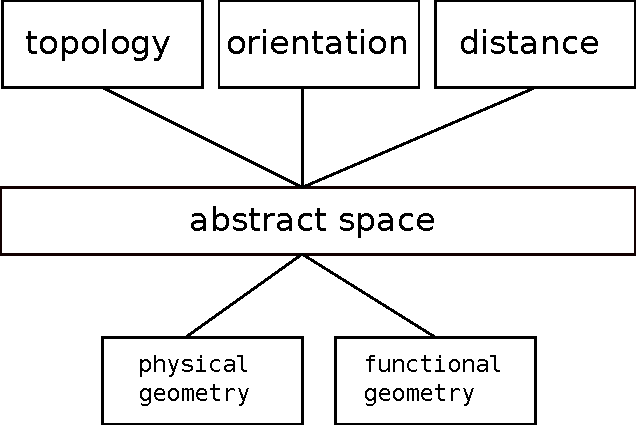
\includegraphics[width=90mm]{reasoner-design}
\caption{Constraint Solvers}
\label{reasoner-design}
\end{figure}

Within the CLP framework of DSpace, the reasoning capabilities are built as a series of spatial constraint solvers using CLP($\mathbb{R}$) (Constraint Logic Programming over Reals) and CHR (Constrain Handling Rules). The spatial constraint solvers work directly over the multiple perspective representation structure via the spatial abstraction representation layer and the design factbase. The main service of the reasoner is qualification of the quantitative architectural space into the qualitative feature space of topology, orientation, and distance. It should be noted that the distance constraint solver is different from the topological and orientational constraint solvers because it does not qualify distance relationships, rather it solves minimum distance constraints over quantitative objects. The topological and distance constraint solvers extend The Sindalog spatial constraint solver \cite{Sindalong}, a spatial constraint solver written in CHR. These qualitative spatial relationships are, in turn, used to reason about conceptual design requirements.

\subsection{Topology}
The DSpace reasoner can qualify the following four topological relationships for convex hulls: inside (\ref{inside}), outside (\ref{outside}), partially overlapping (\ref{overlapping}), and disconnected (\ref{disconnected}). In DSpace topological qualification uses geometric properties of convex hulls to detect topological relationships. 

\begin{figure}[t]
 \centering
 \subfloat[inside]{\label{inside}
\includegraphics[width=27mm]{ntpp}}
 \hspace{4 mm}
 \subfloat[outside]{\label{outside}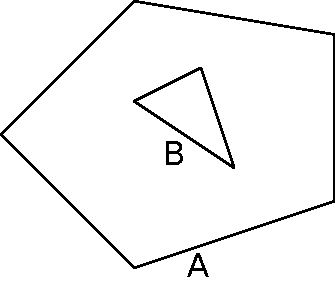
\includegraphics[width=27mm]{ntppi}}
  \hspace{4 mm}
 \subfloat[overlapping]{\label{overlapping}
\includegraphics[width=34mm]{overlapping}}
 \hspace{2 mm}
 \subfloat[disconnected]{\label{disconnected}
\includegraphics[width=43mm]{disconnected}}
 \caption{Topological Relationships}
\label{topoloy}
\end{figure}

An object \emph{A} has an inside relationship with an object \emph{B} if all \emph{A}'s points are inside the convex hull of \emph{B}. The inside relationship is qualified in DSpace by checking the property of convex hull / point containment. A point in \emph{A} is inside the convex hull of \emph{B} if the polarity of the determinate between the point in \emph{A} and each line segment in \emph{B} is negative. Because points in a convex hull are always ordered counterclockwise, in the DSpace representation, the polarity of the determinant between a point inside the convex hull will always be negative. 

An object \emph{A} has an outside relationship with an object \emph{B} if all \emph{B}'s points are inside the convex hull of \emph{A}. Because the outside relationship is the inverse of the inside relation it is easy to qualify in DSpace by using the inside relationship ($inside(B,A)$). 

An object \emph{A} has a partially overlapping relationship with an object \emph{B} if one or more line segments in \emph{A} intersect with one or more line segments in \emph{B}. The partially overlapping relationship is qualified in DSpace by checking for line segment intersection between objects. Two objects are partially overlapping if they intersect in at least one point.  

An object \emph{A} has a disconnected relationship with an object \emph{B} if \emph{A} does not intersect with \emph{B}, there are no points in \emph{A} that are inside \emph{B}, and there are no points in \emph{B} that are inside \emph{A}. The disconnected relationship is qualified by checking for line segment intersection and convex hull / point containment. If there are no line segment intersections and no convex hull / point containment relationships, then two objects are disconnected.  

\subsubsection{Spatial Constraint Solver: Topology}
The topological constraint solver qualifies topological relationships over convex hull objects. Its implementation extends Sindalog's \ref{Sindalog} topological constraint solver by integrating topological constraints over convex hulls. It is written using CHR that simplify and propagate topological constraints into solvable geometric constraints of line segment intersection and convex hull / point containment. Once a constraint is in a solvable form, in this case a line intersection or convex hull / point containment constraint, it is solved and returns true or false based on the outcome of the solution. The topological constraint solver is based on successively breaking down a spatial object (convex hull) or spatial primitive (line, point) until solvable geometric constraints can be checked.

For example, qualification for the partially overlapping topological relationship requires simplifying the overlapping constraint into line segment intersection constraints between the line segments of the convex hulls. The overlapping constraint is solved when at least one line intersection constraint is solved to true or when there are no more line intersection constraints left in the constraint store. In the former case the constraint returns true and in the latter case returns a failure. 

A top level constraint recursively breaks down a convex hull into its line segments and propagates new constraints for line segment to convex hull intersection. The line segment to convex hull intersection constraint further propagates new constraints that check for line segment to line segment intersection. These constraints are the lowest level constraints and are solved when fully instantiated. The following code shows a propagation rule for the overlapping topological relationship for line segment to convex hull intersection. Line segments are represented as a tuple of point, and convex hull are represented as a list of points.   
\begin{verbatim}
   intersect_segment_hull((Pt1, Pt2), [Pt3, Pt4|PS]) <=>
           intersection_segment_segment((Pt1, Pt2), (Pt3, Pt4)),
           intersection_segment_hull(Pt1, Pt2, [Pt4|PS]).
\end{verbatim}
The first constraint \emph{intersection\_segement\_segmenet} is propagated into the constraint store and will be solved when all points in its arguments are fully instantiated. The second constraint is a recursive call that will propagate the \emph{intersection\_segement\_segmenet} constraint for the entire convex hull. 

The qualification for the other topological relationships are similar to the partially overlapping constraint presented here, but in addition to the line intersection constraint some constraints use the geometric properties of convex hull / point containment.

The DSpace design representation structure can be queried for topological relationships using the topological constraint solver. Prolog rules query the abstract representation layer to retrieve the spatial abstractions need for topological qualification. In this case objects will be spatially abstracted into convex hulls. The following rule shows the rule for the inside topological relationship. Note that the rule takes two \emph{dsID} as arguements, queries the abstract representation layer to retrieve the entities convex hull abstract representations, and then makes a finally call to the \emph{inside\_convexhull} constraint.
\begin{verbatim}
    inside(Id1, Id2) :-
            convexhull_abs(Id1, Convex1),
            convexhull_abs(Id2, Convex2),
            insdie_convexhull(Convex1, Convex2).
\end{verbatim}
Given two entities with \emph{dsID}'s \emph{door45} and \emph{room53}, the following query will return true if the entities have an inside topological realtionship and will fail if they do not. In this case they do not have an inside relationship so the query returns fail.
\begin{verbatim}
    ?- inside(door45, room53).
    fail.
\end{verbatim}

\subsection{Orientation} \label{orientation}
The DSpace reasoner can qualify two types of orientational relationships, intrinsic and extrinsic. Intrinsic orientational reasoning is based on OPRA$_{m}$. OPRA$_{m}$ partitions space into half-planes, which are defined by lines emanating from a reference point, and defines the qualitative orientational relationships by the half plane in which a second point is located in relation to the reference point. The granularity of an OPRA$_{m}$ relationship, specified by $m$, defines the number of lines emanating from the reference point. 

\begin{figure}[H]
\centering

\includegraphics[width=60mm]{facing-opra-base-rel}
\caption{OPRA$_{2}$ Space Partitioning}
\label{facing-opra-base-rel}
\end{figure}

Figure \ref{facing-opra-base-rel} shows the OPRA$_{2}$ (two lines) partitioning of space, with labels for the base OPRA$_{2}$ relationships. Point \emph{A} is located in half-plane 7 of point \emph{B}'s partitioned space, and \emph{B} is located in half-plane 1 of \emph{A}'s partitioned space. Note that the arrow depicts the point's direction and the half-planes are labeled starting at the point's direction, incrementing counter-clockwise. 

OPRA$_{m}$ relationships are qualified by solving linear inequalities that are defined by lines emanating from the reference point. Given a point \emph{A} and \emph{B}, the $\theta_{AB}$ symbol refers to $ \tan^{-1} \frac{B_{y} - A_{y}}{B_{x} - A_{X}} $, the $\phi_{A}$ symbol refers to the direction of point \emph{A}, and the \emph{m} symbol refers to the granularity of the OPRA$_{m}$ relations. Equation \ref{opra-eq} shows the linear inequalities that qualify OPRA$_{m}$ relationships as referenced from point \emph{A} to point \emph{B}. Using this system of linear inequalities, the OPRA$_{m}$ relationship ($i$) can be solved for \emph{B} in terms of \emph{A}'s OPRA$_{m}$ space.

\begin{equation}\label{opra-eq}
\begin{aligned}
\Big(&\Big(\Big(\frac{i}{2} \, \in \, N \wedge i < 2\Big) \wedge \Big(2\pi - \frac{i-2}{4m} < \theta_{AB} - \phi_{A} < \frac{2\pi}{4m}\Big)\Big) \\
\lor \;\; \Big(&\Big(\frac{i+1}{2} \in N \wedge i \geq 1\Big) \wedge \Big(\theta_{AB} - \phi_{A} = 2\pi \frac{i-1}{4m}\Big)\Big)\Big) \\ \\
\end{aligned}
\end{equation}

Extrinsic orientational reasoning is based on the SCC. SCC defines the orientation of a point C (referent) with respect to a point B (relatum) from the viewpoint of a point A (origin).

\begin{figure}[H]
\centering
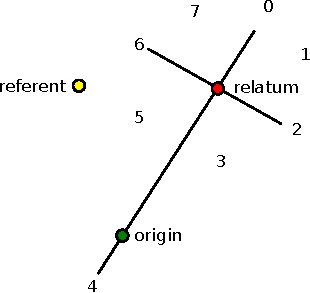
\includegraphics[width=60mm]{scc}
\caption{SCC Partitioning}
\label{scc}
\end{figure}

Figure \ref{scc} shows an SCC relationship between three points. The partitioning scheme is based on the orientation of the origin and relatum points. In this example, the third point, the referent, is located in half-plane 5 of the SCC partitioned space, so it has an SCC$_{5}$ relationship with point \emph{A} as related by \emph{B}. 

\begin{equation}\label{scc-eq} 
\begin{aligned}
\Big(&\Big(\Big(A_{y} < B_{y}\Big) \wedge \Big(C_{y} > M_{perp} \cdot C_{x} + Y_{perp}\Big)\Big) \; \lor \\
\Big(&\Big(A_{y} > B_{y}\Big) \wedge \Big(C_{y} < M_{perp} \cdot C_{x} + B_{perp}\Big)\Big)\Big) \\
\wedge \;\; \Big(&\Big(\Big(A_{x} < B_{x}\Big) \wedge \Big(C_{y} < M_{AB} \cdot C_{x} + B_{AB}\Big)\Big) \; \lor \\
\Big(&\Big(A_{x} > B_{x}\Big) \wedge \Big(C_{y} > M_{AB} \cdot C_{x} + B_{AB}\Big)\Big)\Big) \\
\end{aligned}
\end{equation}


SCC relationships are qualified by solving a system of linear inequalities, which are based on the lines that partition space into the SCC half-planes. Labeling starts at the line that runs between the origin and relatum, starting at zero and incrementing clockwise. Given three points A, B, and C, $M_{AB}$ refers to the slope of line from A to B, $Y_{AB}$ refers to the y-intercept of the line from A to B, $M_{perp}$ refers to the slope of the line that is perpendicular to the line from A to B, and $Y_{perp}$ refers to the y-intercept of the line that is perpendicular to the line from A to B. Given a point \emph{C}, it has an SCC$_{1}$ relationship with points \emph{A} and \emph{B} if the equations in \ref{scc-eq} can be solved. If the equations are not solvable then \emph{C} does not have an SCC$_{1}$ relationship with \emph{A} related to \emph{B}. There are similar systems of inequalities for each of the seven SCC relationships.  


\subsubsection{Spatial Constraint Solver: Orientation}
The orientational constraint solver qualifies OPRA$_{m}$ and SCC relationships over points and directed points. It is written in CLP($\mathbb{R}$) and uses constraints over linear inequalities (Equations \ref{opra-eq}, \ref{scc-eq}) to solve orientational qualification problems. Within the orientational solver there are two modules, one for intrinsic relationships based on OPRA$_{m}$ and one for extrinsic relationships based on SCC.

The OPRA$_{m}$ constraint solver solves extrinsic orientation qualification problems by constraining the linear inequalities in Equation \ref{opra-eq}. Given an origin point \emph{A}, a reference point \emph{B}, and a granularity $m$, the constraint solver will return the OPRA$_{m}$ relationship ($i$) between \emph{A} and \emph{B}. The linear inequalities are constrained as CLP($\mathbb{R}$) constraints and return once all variables in the linear inequalities are instantiated. 

The SCC constraint solver solves intrinsic orientation qualification problems by constraining the linear inequalities in Equation \ref{scc-eq}. Given an origin, a relatum and a referent, the SCC constraint solver will return true or fail based on the resolvability of the linear inequalities. The linear inequalities are constrained as CLP($\mathbb{R}$) constraints and will return true if the linear equalities are solvable and fail if they are not.

The DSpace design representation structure can be queried for orientational relationships using the orientational constraint solver. Prolog rules query the abstract representation layer and retrieve the spatial abstractions need for orientational qualification: point and directed point. The following rule shows the rule for the SCC$)_{1}$ relationship.
\begin{verbatim}
    SCC1(Id1, Id2, Id3) :-
            point_abstraction(Id1, PtAbs1),
            point_abstraction(Id2, PtAbs2),
            point_abstraction(Id3, PtAbs3),
            SCC(PtAbs1, PtAbs2, PtAbs3, 1).
\end{verbatim}
Given three entities with \emph{dsID}’s \emph{door45}, \emph{room53}, and \emph{desk2} the following query will return true if the entities have an SCC$_{1}$ relationship and will fail if they do not. In this specific case they do have an SCC$_{1}$ relationship so the query returns true.
\begin{verbatim}
    ?- SCC1(door45, room53, desk2).
    true.
\end{verbatim}



\subsection{Distance}
The DSpace reasoner can calculate the minimum euclidean distance between points, lines, and polygons. Given two objects the minimum distance is calculated by finding the closest point in each object to the other object. Base on these two point the minimum euclidean distance is calculated. 

\begin{figure}[H]
\centering
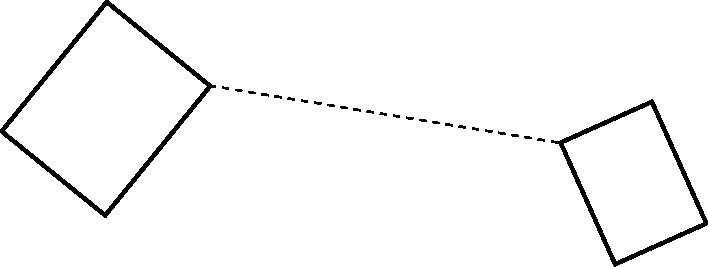
\includegraphics[width=80mm]{min-dist}
\caption{Minimum Distance}
\label{min-dist}
\end{figure}

\subsubsection{Spatial Constraint Solver: Distance}
The distance constraint solver solves minimum distance constraints and uses the distance constraint services of the Sindalog \cite{sindalog} reasoner for its reasoning. The distance solver is different from the other solvers because it returns a value to a query. For example, the following query will return the minimum distance between the two objects in D.
\begin{verbatim}
   min_distance(obj1, obj2, D). 
\end{verbatim}

The distance constraint solver is written using CHR that break down the constraints until they can be solved for. This process involves finding the located on each object that is the closest to the other, so that the minimum distance can be calculated between the two. 


\chapter{Conceptual Requirements Reasoner}
This chapter presents the conceptual requirements reasoning framework of the DSpace reasoner. It shows how architectural concepts and qualitative spatial attributes found in architecture (QSA) can be spatially interpreted using formal qualitative spatial calculi and shows how they can be represented and reasoned with to validate conceptual design requirements in the conceptual requirements reasoner (CCR). 

Conceptual design requirements were ascertained from literature on architectural design \cite{tbd}, museum research on visitor behavior \cite{tbd}, and building regulations and codes \cite{tbd}. Their definitions are explicit characterizations of architectural concepts and spatial design qualities that are based on heuristic architectural knowledge and common sense notions of spatial relationships. The objective is not to be an exhaustive discussion of these requirements or a validation for their interpretation in terms of a spatial or design perspective; rather it is to demonstrate how each can be represented and reasoned with in the DSpace CLP framework to validate conceptual design requirements against the quantitative form of a design. 

In the DSpace CLP framework, QSA and architectural concepts utilize the DSpace design representation structure, via the spatial abstraction layer, and the DSpace spatial reasoner to validate conceptual design requirements. QSA and architectural concepts are implemented as Prolog rules. Each rule is implemented as a conjunction of predicates that spatially define the QSA and architectural concepts from a qualitative perspective. Conceptual design requirements can be specified using QSA, architectural concepts, and qualitative spatial relationships. Validating a design requirement happens by making a Prolog query to the CCR that will return \emph{true} if the design is consistent per the requirement or \emph{fail} if the design is inconsistent per the requirement. 

The chapter is structured as follows: Section 1 presents a set of qualitative spatial attributes found in architecture, shows how each can be interpreted using formal qualitative spatial calculi, and represented formally within DSpace CRR. Section 2 presents a set of architectural concepts that are built using the spatial qualities presented in the Section 1 and shows how they can be used to reason about design requirements within the DSpace CRR. Section 3 shows how conceptual design requirements can be validated in using the CRR.


\section{Qualitative Spatial Attributes found in Architecture}
This section presents a set of qualitative spatial attributes found in architecture (QSA) and shows how each QSA is spatially interpreted and represented in DSpace. QSAs are architectural qualities that emerge from the spatial structures that form from the physical elements of the building (doors, walls, columns, windows, etc.), artefactual extensions (functional space, operational space, range space, etc.) and interior design elements (furniture, lights, decorations, etc.). QSAs can be perceptual qualities that are described from a specific vantage point, or intrinsic qualities that are inherent in the build's spatial structure. 

This section presents five QSAs: positioning, positioning for sequences, facing, visibility, and proximity. The goal of this section is to develop a tool-kit of QSAs that qualitatively describe architectural designs in the spatial environments in which they emerge. Some boundary cases are identified and handled, but it is not the purpose here to explore all possible case scenarios.

\subsection{Positioning}
The positioning attribute defines an orientational relationship between a pair of objects as each object relates to the other within an extrinsic context, i.e., a defined space such as a room, apartment, building, or user defined space. There are four positioning relationships using this scheme: opposing-side of space, same-side of space, left-side of space, and right-side of space. The opposing-side and same-side relationships can be combined, via conjunction, with the left-side or right-side relationships to form the following compound relationships: opposing-left-side, opposing-right-side, same-left-side, same-right-side.

\begin{figure}[H]
\centering
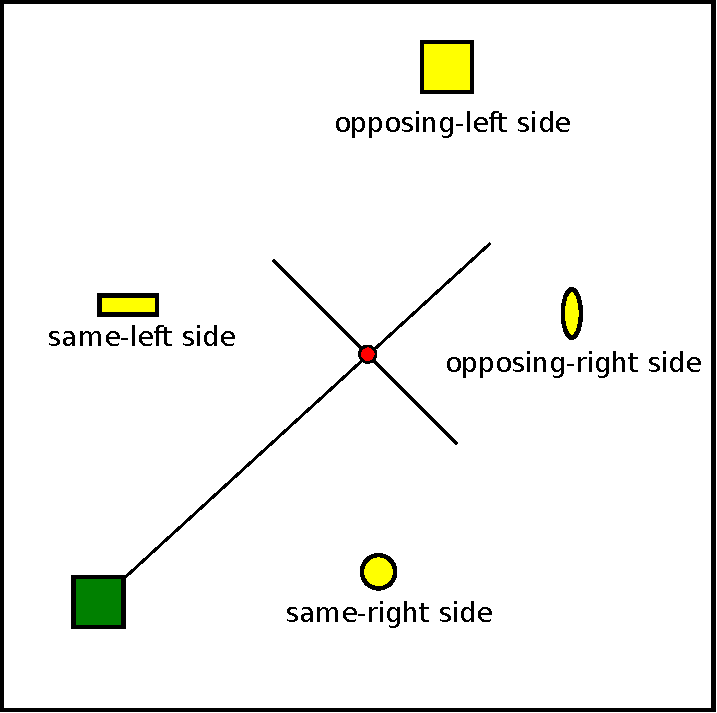
\includegraphics[width=80mm]{position}
\caption{Positioning}
\label{position}
\end{figure}

The positioning attribute is interpreted spatially, in DSpace, using the Single Cross Calculus (SCC) \cite{Freksa92usingorientation}. SCC defines the orientation of a point C (referent) with respect to a point B (relatum) from the viewpoint of a point A (origin). The positioning attribute uses the SCC partitioning scheme to orientationally relate two points (origin, referent) in the context of an external frame of reference (relatum). In DSpace, the reference point is defined as the centroid of the context space. By partitioning space using the centroid, an approximation is made that divides the space into the positioning relationships. An assumption made in DSpace is that the space will generally be rectangular in shape.

\begin{figure}[H]
\centering
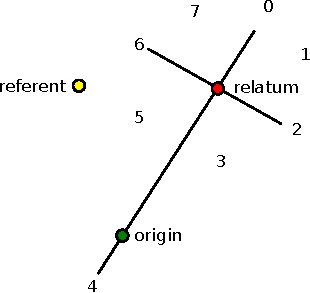
\includegraphics[width=60mm]{scc}
\caption{SCC Partitioning}
\label{scc}
\end{figure}

Under this scheme, two points are defined as being on opposing sides of a space if they have an SCC relationship of 0, 1 or 7, as related by the centroid of the space. Conversely, a pair of points are defined as being on the same side of a space if they have an SCC relationship of 3, 4 or 5, as related by the centroid of the  space. A point is defined as being on the left side of a space from another point if it has an SCC relationship of 5, 6, or 7, and is on the right side if it has an SCC relationship of 1, 2, or 3. Using the union set operation these relationships can be combined to form the opposing-left/right, and same-left/right relationships.

Th positioning relationships are represented in the DSpace CLP framework as Prolog rules. There is a single rule for each relationships: opposing side, same-side, left-side, and right-side. The head of each rule takes three arguments, the first two for the architectural objects being related and one for the context space. The body of the rule ....  The following is Prolog code for the positioning rules.
\begin{verbatim}
   opposing_side(Obj1, Obj2, Context) :- 
           centroid(Context, Centroid),
           (scc(Obj1, Centroid, Obj2, 0);
            scc(Obj1, Centroid, Obj2, 1);
            scc(Obj1, Centroid, Obj2, 7)).
                                          
   same_side(Obj1, Obj2, Context) :- 
           centroid(Context, Centroid),
           (scc(Obj1, Centroid, Obj2, 2) ;
            scc(Obj1, Centroid, Obj2, 3) ;
            scc(Obj1, Centroid, Obj2, 4) ;
            scc(Obj1, Centroid, Obj2, 5) ;
            scc(Obj1, Centroid, Obj2) 6)).   

\end{verbatim}

The positioning attribute can be used to check if architectural structures, artefactual extensions, or interior design elements are on the opposing or same side of a space to the other. For example, a requirement might state that a bedroom should be positioned to the back of a house from the main entrance. The reason for this requirement is that rooms that are in the back of a house are more private than rooms in the front of the house. In this requirement, the origin is the entrance, the referent is the bedroom, and the relatum is the centroid of the house (context space). 
\begin{figure}[H]
 \centering
 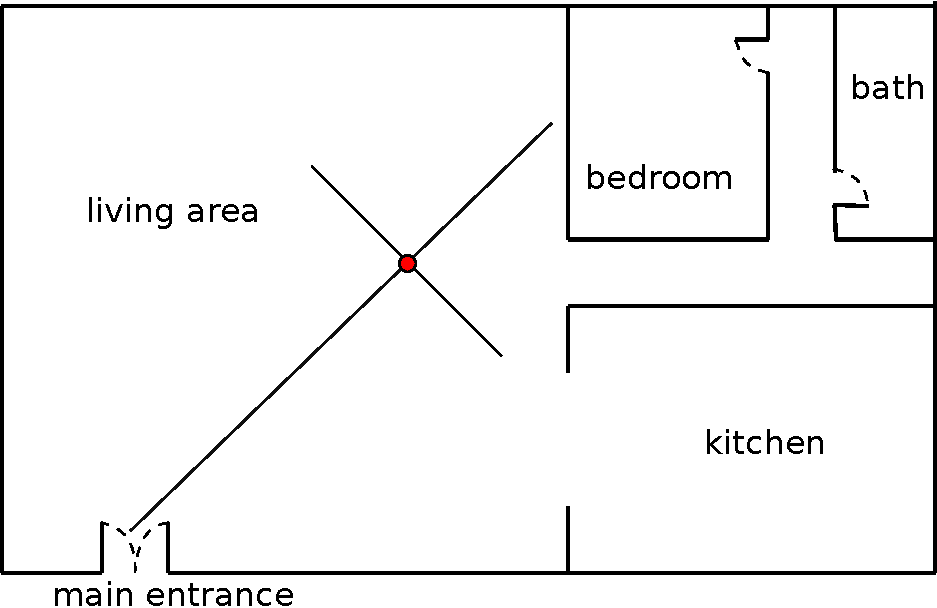
\includegraphics[width=95mm]{bedroom-back-house}
 \caption{Bedroom Privacy}
\label{privacy}
\end{figure}



\subsection{Positioning for Sequences}
The positioning for a sequences attribute defines a perceptual orientational relationship of a sequence of objects as each relates to a vantage point in an extrinsic context, i.e., a defined space such as a room, apartment, building, or user defined space. A sequence is a set of architectural entities (columns), or interior design objects (display cases) that are grouped together and comprised of the same entity or object type. In general sequences are grouped together based on the proximity of the objects (near to each other) but any relationship can define a sequence. There are three positioning relationships for a sequence of objects: horizontal perceived, vertical perceived, and neither.  

The positioning for a sequence of objects attribute can be spatially interpreted using SCC, similar to the positioning attribute above. The positioning for a sequence of objects attribute uses the SCC partitioning scheme to orientationally relate a sequence of points (origin, referents) in the context of an external frame of reference (relatum). In DSpace, the reference point is defined as the centroid of the context space. By partitioning space using the centroid, an approximation is made that divides the space into the positioning relationships. As with the positioning attribute, an assumption made in DSpace is that the space will generally be rectangular in shape.

Using the SCC partitioning of space, a sequence of objects is perceived horizontally from the vantage point if the sequence of points have the following combination of SCC relationships (origin = vantage point, relatum = context centroid, referent = sequence point): at least one point in the sequence has an SCC$_{5}$ or SCC$_{6}$ or SCC$_{7}$ relationship and at least one point has an SCC$_{1}$ or SCC$_{2}$ or SCC$_{3}$ relationships. A sequence of points is perceived vertically if they have the following combination of SCC relationships: at least one point in the sequence has an SCC$_{5}$ or SCC$_{3}$ relationship and at least one point in the sequence has an SCC$_{0}$ or SCC$_{1}$ or SCC$_{7}$ relationship. Sequences can be both vertical and horizontal at the same time or they can be neither. The neither relationship is defined by a sequence of object that do not match any of the sets above.

TODO: figures

Th positioning for a sequence of objects relationships are represented in DSpace as Prolog rules. There is a single rule for each relationship: horizontally perceived, vertically perceived, diagonally perceived, and . The head of each rule takes three arguments, the first for the the vantage point, the second is a list of objects that represent the sequence and the third is the context space. The body of the rule .... Given a vantage point, a sequence of objects and a context space, the rule returns true if the objects are on the horizontally perceived, vertically perceived, diagonally perceived, or confined as defined by its' rule, and fails if they are not. The following is Prolog code for the positioning rules.
\begin{verbatim}
   horizontally_perceived(vantage_point, seq_list, context) :-
           centroid(context, Centroid),
           horizontally_
\end{verbatim}


\subsection{Facing}
The facing attribute defines an intrinsic orientational relationship between two objects as each object relates to the other. The definition used here is based on a common sense interpretation of facing, in which an object \emph{A} is facing towards an object \emph{B}, if \emph{A} is directionally oriented at \emph{B}. Under this definition, a pair of objects can be facing towards or away from each other. Given a pair of objects, \emph{A} and \emph{B}, there are four possible facing configurations between the pair: 

\begin{figure}[H]
 \centering
 \subfloat[A, B towards]{\label{fig:facing-towards}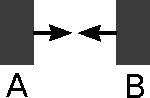
\includegraphics[width=25mm]{facing-towards}}
 \hspace{10 mm}
 \subfloat[A, B away]{\label{fig:facing-away}
\includegraphics[width=28mm]{facing-ABaway}}
  \hspace{10 mm}
 \subfloat[A towards, B away]{\label{fig:facing-A}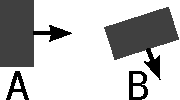
\includegraphics[width=28mm]{facing-Atowards-Baway}}
 \hspace{10 mm}
 \subfloat[A away, B towards]{\label{fig:facing-A}
\includegraphics[width=28mm]{facing-Aaway-Btowards}}
 \caption{facing}
\label{display-arrangement}
\end{figure}

The facing attribute is spatially modelled in DSpace using the Oriented Point Relation Algebra \cite{Moratz} (OPRA). The advantage of using OPRA is that it models the intrinsic orientational relationships between a pair of directed points. TODO: mention something about the section that talks about OPRA. Using OPRA$_{8}$, the facing attribute can be defined in terms of the half plane sectors. Point \emph{A} is facing towards point \emph{B}, if \emph{B} is located in sectors 0, 1, or 32 of \emph{A}'s partitioned space. Similarly, if \emph{A} is located in sectors 0, 1, or 32 of \emph{B}'s partitioned space then \emph{B} is facing towards \emph{A}. In this case, both points are facing towards each other. Conversely, point \emph{A} is facing away from point \emph{B} if \emph{B} is located in sectors 2 - 31 of \emph{A's} partitioned space. A granularity of 8 is used (i.e., OPRA$_{8}$) to define a narrow interpretation of the facing attribute. Within a room, doorways, windows, and walls are generally face towards each other. By narrowing the space that is considered facing towards, it allows DSpace to detect elements that are more directly facing towards each other.

Figure \ref{fig:facing-opra-towards} shows an example of two points facing towards each other; note that each point is located in sector 32 of the other's partitioned space.  Figure \ref{fig:facing-opra-away} shows an example of two points that are facing away from each other and are not located in sectors 0, 1, 32 of the other's partitioned space. 

\begin{figure}[H]
 \centering
 \fbox{
 \subfloat[facing towards]{\label{fig:facing-opra-towards}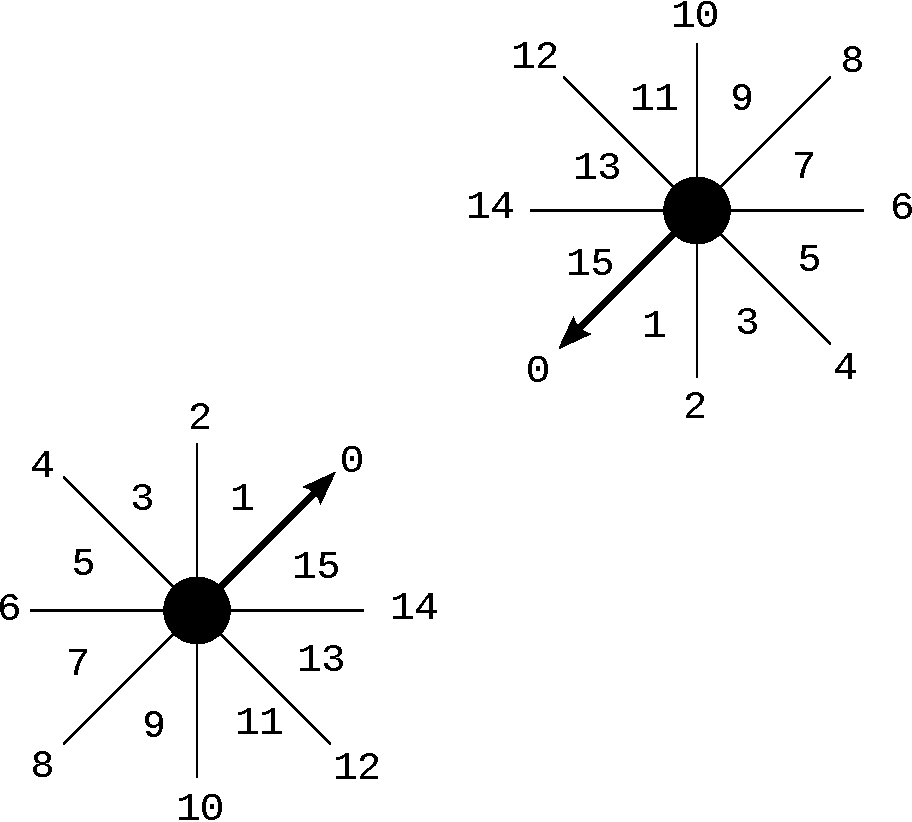
\includegraphics[width=60mm]{facing-opra}}
 }
  \hspace{10 mm}
  \fbox{
 \subfloat[facing away]{\label{fig:facing-opra-away}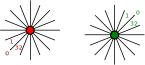
\includegraphics[width=60mm]{facing-away-opra}}
 }
 \caption{OPRA Partitioning }
\label{opra-facing}
\end{figure}

The facing attribute is represented in DSpace as Prolog rules. There is one rule for facing-towards and one for facing-away. The head of each rule takes two arguments for the objects being related. The body of the rule is a single disjunctive clause that checks for the OPRA$_{8}$ relationship between the objects. Given two objects, the rule returns true if the objects are facing towards or away from each other as defined by the rule, and fails if they are not. The following is Prolog code for the facing rules.

\begin{verbatim}
   facing_towards(Obj1, Obj2) :- 
           (opra(Obj1, Obj2, 0) ;
            opra(Obj1, Obj2, 1) ;
            opra(Obj1, Obj2, 32)).
                                 
   facing_away(Obj1, Obj2) :- 
           not facing_towards(Obj1, Obj2).                     
\end{verbatim}

In DSpace, the facing attribute can be used to check if two architectural structures, artefactual extensions, or interior design elements are facing towards or away from each other. For example, doorways and windows that face towards each other promote airflow through the space they inhibit. A design that requires good air circulation could use this knowledge to ensure proper airflow. Figure \ref{door-window-facing} shows two example floor plans of a room with a window and doorway. Figure \ref{fig:door-window-towards} shows a configuration were the doorway and window are facing towards each other, while figure \ref{fig:door-window-away} shows a configuration where the doorway and window are facing away from each other. 

\begin{figure}[H]
 \centering
 \subfloat[facing towards]{\label{fig:door-window-towards}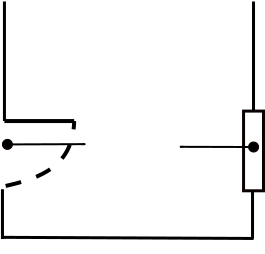
\includegraphics[width=55mm]{door-facing-window-con}}
  \hspace{10 mm}
 \subfloat[facing away]{\label{fig:door-window-away}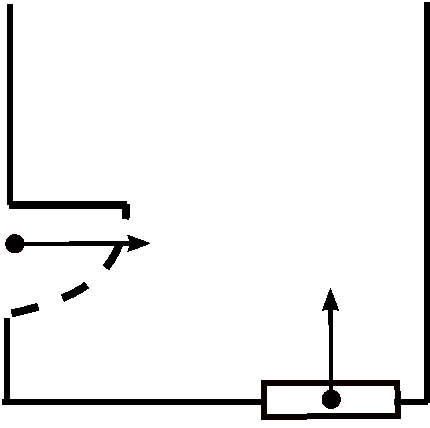
\includegraphics[width=53mm]{door-facing-window-incon}}
 \caption{Door, Window Facing}
\label{door-window-facing}
\end{figure}

Within the context of architecture, care needs to be taken to account for architectural structures that are long in one axis, such as walls, because the spatial abstraction for OPRA is a directed point. This means that an object is defined as facing towards a wall if it is facing towards the wall's directed point abstraction (usually the centroid of the wall). Under this definition, there are configurations where an object should be considered to be facing a wall but it is not. DSpace handles this special case by modifying the OPRA$_{8}$ relationships that correspond to facing towards and away from a wall. 

fig: wall example

\subsection{Proximity}
The proximity attribute defines a qualitative distance relationship between two objects. In DSpace, there are three proximity relationships: near, near+, and far. The spatial interpretation of proximity is defined in the context of architecture, which is restricted here to be \emph{within a building}. Based on this interpretation, proximity is formally defined using heuristics based on what is consider near, near+, and far within a building.   


\begin{figure}[H]
\centering
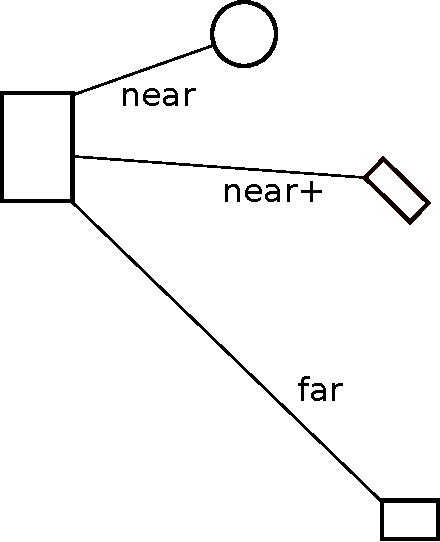
\includegraphics[width=45mm]{proximity}
\caption{Proximity}
\label{proximity}
\end{figure}

Using these heuristics, two objects are near if the minimum distance between them is less then or equal to 3 meters, near+ if the minimum distance between then is between 3 - 6 meters, and far if the minimum distance between them is greater then 3 meters. While the definition of proximity pivots around 3 and 6 meters, it can easily be changed by using an extra parameter in a proximity predicate. 

Proximity is represented in DSpace as three Prolog rules. There is one rule for near, one for near+, and one for far. The head of each rule takes two arguments for the architectural objects being related. The body of the rule .... Given two objects, the rule returns true if the objects are near, near+, or far from each other as defined by the rule, and fails if they are not. The following is Prolog code for the proximity rules.

\begin{verbatim}
   near(Obj1, Obj2) :- 
           minimum_distance_compare(Obj1, Obj2, <=, 3).
   
   near_plus(Obj1, Obj2) :-
           minimum_distance_compare(Obj1, Obj2, <=, 6),
           minimum_distance_compare(Obj1, Obj2, >, 3).   
   
   far(Obj1, Obj2) :- 
           minimum_distance_compare(Obj1, Obj2, >, 6)

\end{verbatim}

The proximity attribute can be used to check whether two architectural structures, artefactual extension, or interior design elements are near or far. For example, a computer desk should be located near a power outlet to make it easy to power up the desk's computer and desk's lamp. Another example is the bathroom should be far away from the kitchen, in order to keep a separation between the two.

\begin{figure}[H]
 \centering
 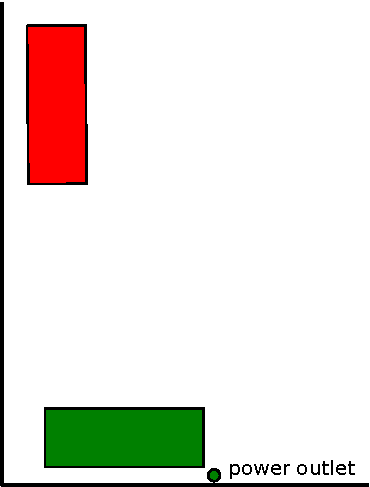
\includegraphics[width=50mm]{desk-proximity}
 \caption{Desk Outlet Proximity}
\label{desk-proximity}
\end{figure}

\subsection{Visibility}
The visibility attribute defines a boolean relationship between a viewpoint and an object with respect to the object being visible from the viewpoint. This interpretation of visibility is based on the topological characteristics of an object blocking (obstructing) a view. It does not take into account the material characteristics of the obstructing object, such as glass, which would allow visibility through the obstructing object. Additionally it does not take into account the effects of distance on visibility, i.e., an object that is very far away is not visible. However, within the context of architecture and buildings, the magnitude of distances is limited to a point that it is not a factor to visibility. Under this definition, an objects is visible if the view-space (i.e., the space between the viewpoint and the object) is not obstructed.

The spatial interpretation of visibility is based on the topological characteristics of the space in-between the viewpoint and object. This space is referred to as the view-space. An object is visible if the view-space is not obstructed by surrounding structures or objects. An obstructing object is an object that has a partially overlapping or containing topological relationship with the view-space. Artefactual extension is not considered as an obstructing object because it does not have a physical form. This definition does not distinguish between visibility that is partially or totally obstructed.

\begin{figure}[H]
 \centering
 \subfloat[obstructed view]{\label{fig:obstructed-view}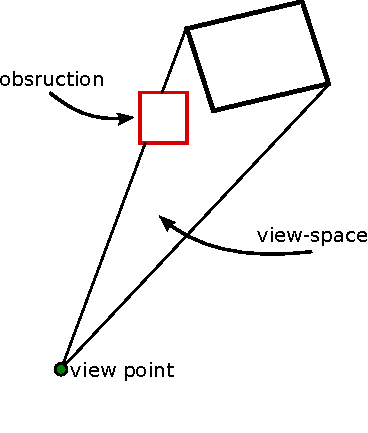
\includegraphics[width=55mm]{visibility}}
  \hspace{10 mm}
 \subfloat[non-obstructed view]{\label{fig:no-obstruction}
\includegraphics[width=55mm]{visibility-no-obstruction}}
 \caption{Visibility}
\label{Visibility}
\end{figure}

Visibility is represented in DSpace as a single Prolog rule. The head of the rule takes two arguments, the viewpoint and the object that is being check for visibility. The body of the clause calculates the view-space and checks the surrounding objects for a topological obstruction. Given a viewpoint and an object, the rule returns true if the object is visible, and fails if it is not. The following is the Prolog code for the visibility rule.

\begin{verbatim}
   is_visible(ViewPoint, Obj) :- 
           view_space(ViewPoint, Obj, ViewSpace),
           topology(ViewSpace, SurroundingStructs).
\end{verbatim}

The visibility attribute can be used to check if an architectural structure or interior design element is visible from a given viewpoint. For example, an architect might want to ensure that a staircase is visible from the main entrance of a building, because she doesn't want the staircase to go unnoticed. Figure \ref{visibility-door-stair} shows an example floor plan where the stairway is not visible from the doorway. In this example both the wall in red and column are obstructing the view from the doorway. 

\begin{figure}[H]
\centering
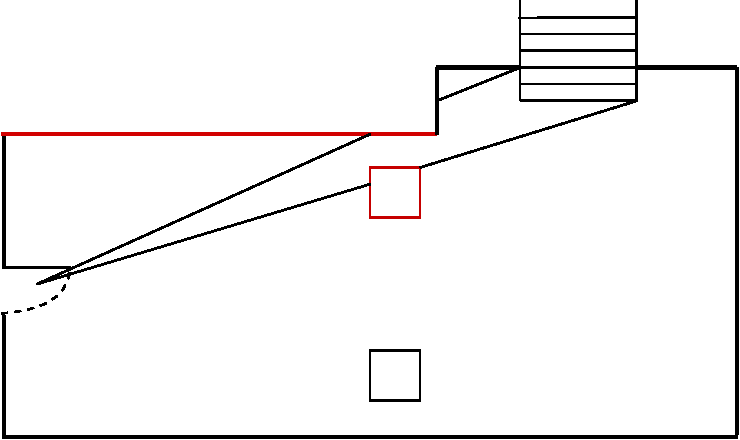
\includegraphics[width=80mm]{visibility-stair-door}
\caption{Visibility Example: Doorway and Stairs}
\label{visibility-door-stair}
\end{figure}



\section{Architectural Concepts}
Architectural concepts, such as privacy, continuity, and enclosure, are experiential aspects of architecture that are used by architects to describe the functionality of a design \cite{Koile}. These terms are defined in DSpace in a hierarchical manner in which architectural concepts are built using QSAs and geometric primitives (orientation, topology, distance). 

This section presents four architectural concepts and demonstrates how each is defined in DSpace. As in the previous section, the purpose is not to investigate the correctness of the concepts or an attempt to compile a complete list, rather it is to look at how these concepts can be defined logically using architectural qualities and spatial / geometric primitives.

\subsection{Privacy}
In architecture, the concept of privacy implies a notion of separation and obscurity (not being visible). In the case of a room, privacy can be defined as being separated from the main entrance of the building and having doorways that enhances the room's privacy. A doorway can be be defined as private with respect to its functionality of connecting two adjacent areas (rooms, hallways, etc.). Under this consideration, a doorway can enhance or hinder the privacy of a room. A doorway enhances privacy of a room if the doorway faces away from other local doorways (doorways in adjacent rooms) and if it is not visible from the main living space. 

Within DSpace, the concept of privacy has been formally defined for rooms and doorways. A door is private if it has the following attributes: (1) it is not visible from the main living space, (2) it does not mutually face towards another doorway and (3) it does not face towards the centroid of an adjacent room. A room is private if it has the following attributes: (1) it is positioned on the opposing side of the building with regard to the main entrance and (2) all doorways into the room are private, per the doorway privacy definition.
 
Privacy is represented in DSpace as Prolog rules. The rules take a single argument, in the head, which indicates if the rule is for a room or doorway. The body of the rule defines the properties of the privacy using QSAs, as defined above. Note that there are two predicates, one for the definition of privacy for a room and one for privacy of a doorway.  

\begin{verbatim}
   private(room) :-  
           opposing_side(room, main_entrance, building), 
           private(doorway).
                     
   private(door) :- 
           facing_away(door, door),
           facing_away(door, adjacent_space),
           not_visible(door, main_living_space). 
\end{verbatim}

Figure \ref{room-privacy} shows two floor plans for a small single bedroom house; figure \ref{fig:private-room-con} shows a floor plan with a bedroom that is  private, while figure \ref{fig:private-room-incon} shows a similar floor plan with a bedroom that is not private. The numbers in the figures represent the following privacy requirements: (1) the bedroom is positioned on the opposing side of the building with regards to the main entrance, (2) the doorway is not visible from the main living space, and (3) the doorway does not mutually face towards another doorway. Numbers that are colored red indicate that the requirement has been broken, while numbers in green indicate that the requirement has been met.

\begin{figure}[H]
 \centering
 \subfloat[Private]{\label{fig:private-room-con}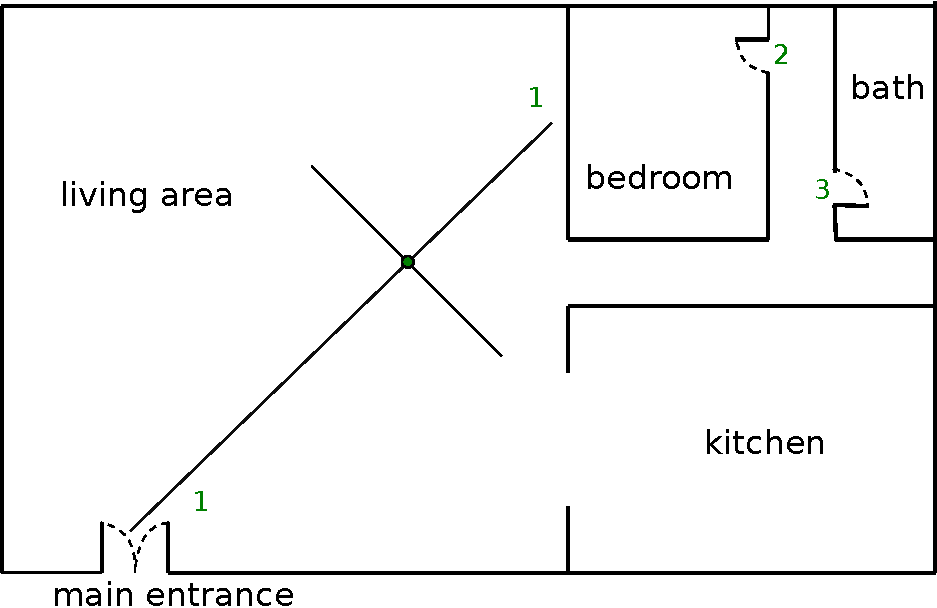
\includegraphics[width=69mm]{privacy-room-con}}
  \hspace{5mm}
 \subfloat[Not Private]{\label{fig:private-room-incon}
\includegraphics[width=69mm]{privacy-room-incon}}
 \caption{Bedroom Privacy}
\label{room-privacy}
\end{figure}

\subsection{Continuity}
In architecture, the concept of continuity describes a network of points that are mutually visible \cite{Key}. In DSpace, continuity is interpreted in the context of building navigation and wayfinding and is therefore dependent on continuity between doorways withing the design. Other interpretations of continuity can use any element of the design (beyond doorways), however for the purposes here, continuity only deals with doorways. Under this interpretation, a building, room or apartment is continuous if there is continuity between the doorways contained in a given space: room, building, or apartment. 

Continuity is defined as a network of doorways that are mutually visible. The partitioning of doorways that should be mutually visible is based on a localized containment hierarchy between rooms and doorways, in which doorways that are contained in the same room should maintain continuity. It does not make sense for doorways that are located on opposite sides of a building to be visible to each other, but doorways that are in the same room should be. 

With respect to this definition, continuity is represented as a recursive rule in Prolog, which takes a list of doorways and checks that each doorway is mutually visible to the others within the list. (need to mention doorways within a room). TBD: arguments: list of doors or room id that indicates containment level???

\begin{verbatim}
   continuous([Obj1,Obj2|[]]) :- 
           is_visible(Obj1, Obj2).

   continuous([Obj1,Obj2|OS]) :- 
           is_visible(Obj1, Obj2),
	       is_visible(Obj2, Obj1),
           continuity([Obj1|OS]),
           continuity([Obj2|OS]).
\end{verbatim}

Figure \ref{continuity} shows a floor plan for a single room with three doors. Figure \ref{fig:continuity-con} shows a configuration in which each door is mutually visible to the other doors. This design is continuous. Conversely, figure \ref{fig:continuity-incon} shows a configuration in which door 1 is not mutually visible to door 2 and door 1 is not mutually visible door 3. The visibility between door 1 and door 2 is obstructed by a column and the visibility between door 1 and door 3 is obstructed by a wall. Structural elements that are colored red indicated a visibility obstruction. This design is not continuous. 

\begin{figure}[H]
 \centering
 \subfloat[Consistent]{\label{fig:continuity-con}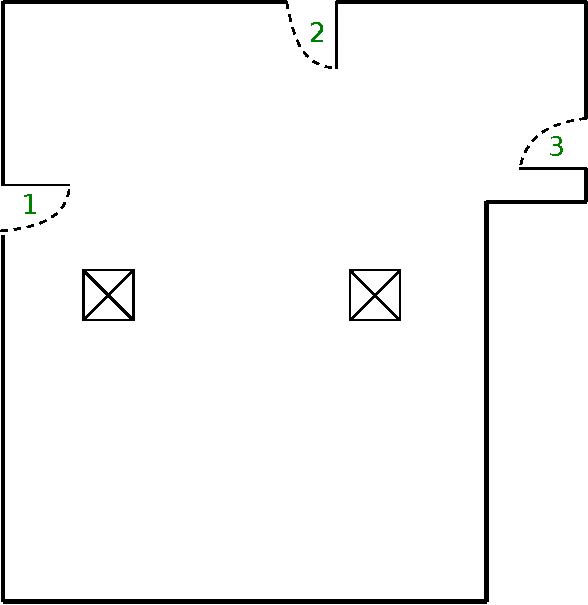
\includegraphics[width=45mm]{continuity-con}}
  \hspace{30 mm}
 \subfloat[Inconsistent]{\label{fig:continuity-incon}\includegraphics[width=45mm]{continuity-incon}}
 \caption{Continuity}
\label{continuity}
\end{figure}

\subsection{Enclosure} 
In architecture, the concept of enclosure defines a space, as experienced from a given vantage point, as being confined or open. A tbdspace space is defined as being confined by walls or columns, while an open space is defined as being spacious. In DSpace, enclosure is defined by localized spatial structures in terms of their proximity to a given point. Under this interpretation, a room, apartment, or building can be experienced as both confined and open based on the location of the vantage point within the space. Such a definition takes into account that enclosure is locally experienced. For example, an alcove in an otherwise open room, feels confined when experienced from inside the alcove.

In Dspace, a point is defined as open if less then three walls or columns are near-to the point. Conversely, a point is defined as confined if three or more walls or columns are near-to the point. While this interpretation of enclosure is naive, it maintains the notion that proximity defines the spatial structures of openness and confinement in a localized environment.   

\begin{verbatim}
confined(point) :-  

spacious(point) :-

\end{verbatim} 

Figure \ref{enclosure} shows a floor plan for a single room with various enclosure properties. The room contains an alcove and a sequence of columns that will provide an environment of confinement. Points in-between the columns and inside the alcove are confined because of the proximity of the walls and/or columns. The points outside of these areas are open because there are few structures nearby.

\begin{figure}[H]
\centering
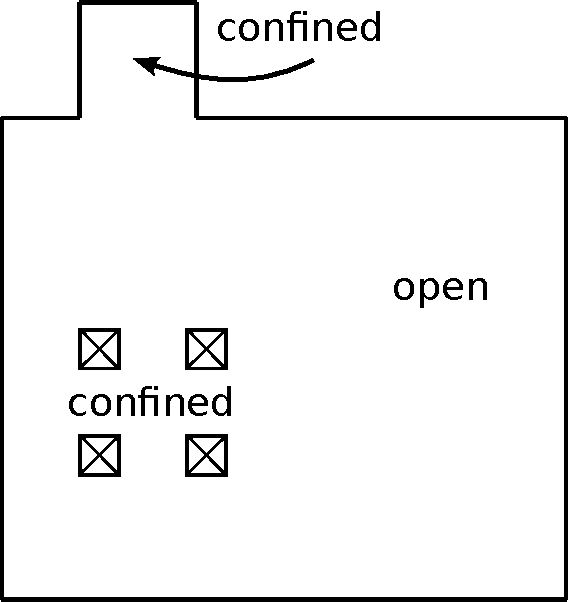
\includegraphics[width=60mm]{spacious-confined}
\caption{Enclosure, Confined and Open}
\label{enclosure}
\end{figure}


\subsection{Artefactual Requirements}
Artefactual requirements are a special case in this section because they are not strictly architectural concepts. However, they provide a unique set of architectural requirements that incorporate a breadth of design aspects. This section will take a look at two examples of artefactual interference. 

Artefactual interference deals with the unintentional interactions of the operational and functional spaces of a building's structural form. For example, the operational space of a bathroom doorway that overlaps with the functional space of the bathroom sink will cause circulation problems into and out of the bathroom. In DSpace, this type of interaction can be detected using topological reasoning over the artefactual extensions of the entities. 

\begin{figure}[H]
\centering
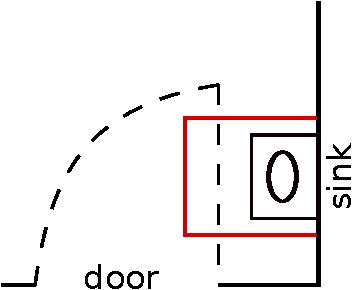
\includegraphics[width=50mm]{door-sink}
\caption{Sink Doorway Interference}
\label{door-sink-example}
\end{figure}

This type of artefactual interaction can be checked for in DSpace using a single rule that takes two arguments in the head of the rule. The body of the rule retrieves the artefactual geometry of each element and checks their topological relationship. It fails if the artefacts have an overlapping relationship.

\begin{verbatim}
   bathroom_sink_door(sink, door) :- 
           artefact_geometry(sink, Artefact_sink),
           artefact_geometry(door, Artefact_door),
           not_overlapping(Artefact_sink, Artefact_door).
\end{verbatim}

Artefactual interactions can be between a physical structure (door, wall, column, ect.) and artefactual extension. For example, the landing space (operational space in DSpace parlance) of a stair should be clear. Representing this requirement is similar to the bathroom sink example except that it checks for interactions between the stair's artefactual space with the building physical space.

In DSpace this can be represented as a single rule. The body of the rule checks for an overlapping relationship between the landing space of the stair and both the artefactual extension and physical structure of surrounding elements.

TBD: figure of stair landing

\begin{verbatim}
    clear_stair_landing(stair, Obj) :- 
            artefact_geometry(stair, Artefact_stair),
            artefact_geometry(Obj, Artefact_obj),
            physical_geometry(Obj, Physical),
            not_overlapping(Artefact_stair, Artefact_obj),
            not_overlapping(Artefact_stair, Physical)
\end{verbatim}  

\section{Conceptual Requirement Validation}
The conceptual requirement reasoner (CCR) validates design requirements by querying an architectural design using predicate calls to architectural concepts and QSA. Requirement queries will return \emph{true} if the architectural design is consistent, or \emph{fail} if the design is inconsistent per the design requirement. A design is considered consistent if the design's spatial characteristics, as represented in its physical and functional geometries, matches with the definition of the designs requirement specification. For example, a design is consistent per a design requirement of a window and doorway facing towards each other, if the spatial characteristic of the design, with regards to the window and doorway, match the spatial specification of facing towards each other.    

Given the example scenario above, a doorway with dsID \emph{door543}, and a window with dsID \emph{window15}, the following query is made to the CRR to validate the requirement.
\begin{verbatim}
   ?- facing(door543, window15).
\end{verbatim}
Queries to architectural concepts and QSA can be combined to build requirements. For example, a design requirement for a doorway and window being near each other can be combined with the previous requirement to build a new requirement. This requirement can be queried directly or implemented as a new Prolog rule. 
\begin{verbatim}
   ?- facing(door543, window15),
      near(door15, window15).
      
    facing_and_near(Id1, Id1) :-
            near(Id1, Id2),
            facing(Id1, Id2).
\end{verbatim}
Note that the direct query is specific to \emph{door543} and \emph{window15}, while the rule allows the user to input any \emph{dsID}'s into the query.
\begin{verbatim}
    ?- facing_and_near(desk52, door6).
\end{verbatim}

Consider the design requirement for a bedroom being private. This requirement can be validated for a design by querying the privacy predicate, as demonstrated above. However, this definition of privacy might not be enough for a particular user. In DSpace, the user can easily extend the definition of privacy by building new Prolog rules that join additional architectural concepts, QSA, and spatial qualities to the existing definition. If the user wants the definition of privacy to include an additional requirement that the bedroom is far away from the living room, the user can construct a new rule by joining the privacy predicate with the proximity predicate. The following is the new predicate for privacy:
\begin{verbatim}
    privacy_new(IdRoom, IdLivingRoom) :-
            privacy(IdRoom),
            far(IdRoom, IdLivingRoom).
\end{verbatim}



\chapter{Case Studies}
This chapter is a case study that demonstrates the application of the DSpace reasoner to the design of an art museum. The purpose is twofold: first, to examine several design requirements of an art museum with regards to the spatial interpretation of the requirements; and second, to show how the museum design requirements can be represented and reasoned about in a computational framework, in order to detect design inconsistencies as per the design requirements.

The remainder of the chapter is divided into three sections. The first section examines design requirements in art museums in three parts: the first part looks at requirements that influence museum visitors' behaviour. The second part looks at requirements for promoting exploration in the museum. The third part looks at the requirements of accessibility and security within the museum. The second section, looks at how these requirements can be interpreted spatially and represented in the DSpace reasoner. The third section tests the DSpace reasoner using sample museum floor plans that are both consistent and inconsistent per the design requirements for several art museums. The objective of this demonstration is to show that the DSpace reasoner can validate a design against its design requirements.


\section{Case Study: Museum}
Museums are a place of public education, in which art, historical artefacts, and scientific exhibits are put on display for the public to view \cite{Falk}. While museums in general have many common threads in terms of their design requirements, this case study takes the approach of narrowing the study to that of an art museum. This focuses the discussion to specific real world examples and maintains the perspective that this is not an exhaustive study of museum design requirements, rather it's an investigation into the nature and interpretation, with respect to spatial properties / characteristics, of a set of design requirements. Additionally, the point is not to prove the validity of these requirements in an empirical sense; rather it is to show the process of representing and reasoning about design requirements in a formal computational framework.

The art museum is a unique and fruitful choice for this case study because it provides a rich set of design properties that have been formally studied and reported \cite{Melton} \cite{Bitgood02} \cite{Falk}. Within museum studies, visitor behaviour has been one of the primary focuses, starting with experiments dating back to the 1930's. 

\subsection{Museum Design Requirements}
Pretend for a moment that you are an architect working on the initial design for a new modern art museum. During your first visit with the museum's curator you discuss several design requirements that are important for the new museum. Your discussion reveals that the curator wants the new art museum to adhere to the following requirements:

\begin{enumerate}
\item Maximize visitor utilization of exhibitions
\item Encourage free-flowing exploration throughout the museum
\item Adhere to museum requirements of accessibility and security
\end{enumerate}

TBD: explain how these high level requirements can be interpreted into concrete properties of the museums design. from here the requirements can be spatially interpreted and represented in the DSpace reasoner.

\subsection{Maximizing Visitor Utilization of Exhibitions}
This portion of the case study will look into four factors that influence visitors' movement patters: positioning of doorways, spatial arrangement of display cases, positioning of furniture and statues, and congestion. These properties inform museum architects, during the design process, about the spatial characteristics that can maximize the utilization of the museum by increasing the frequency and duration with which visitors view exhibition objects. 

\subsubsection{Positioning of doorways}
In an important study, Melton \cite{Melton} discovered that the most influential factor to determine  the amount of attention an exhibition piece receives is the pieces's position relative to doorways in a gallery room. Prior to this, museum researchers believed that the pieces's intrinsic properties of 'interestingness', color, and size were the real factors that determined the amount of attention a piece received. Melton explained why this happens; he demonstrated that the amount of attention a piece receives is directly related to the visitor circulation patterns within the museum and these circulation patterns emerge from the spatial characteristics of the museum's architecture.

\begin{figure}[H]
 \centering
 \subfloat[circulation pattern]{\label{fig:door-opposite}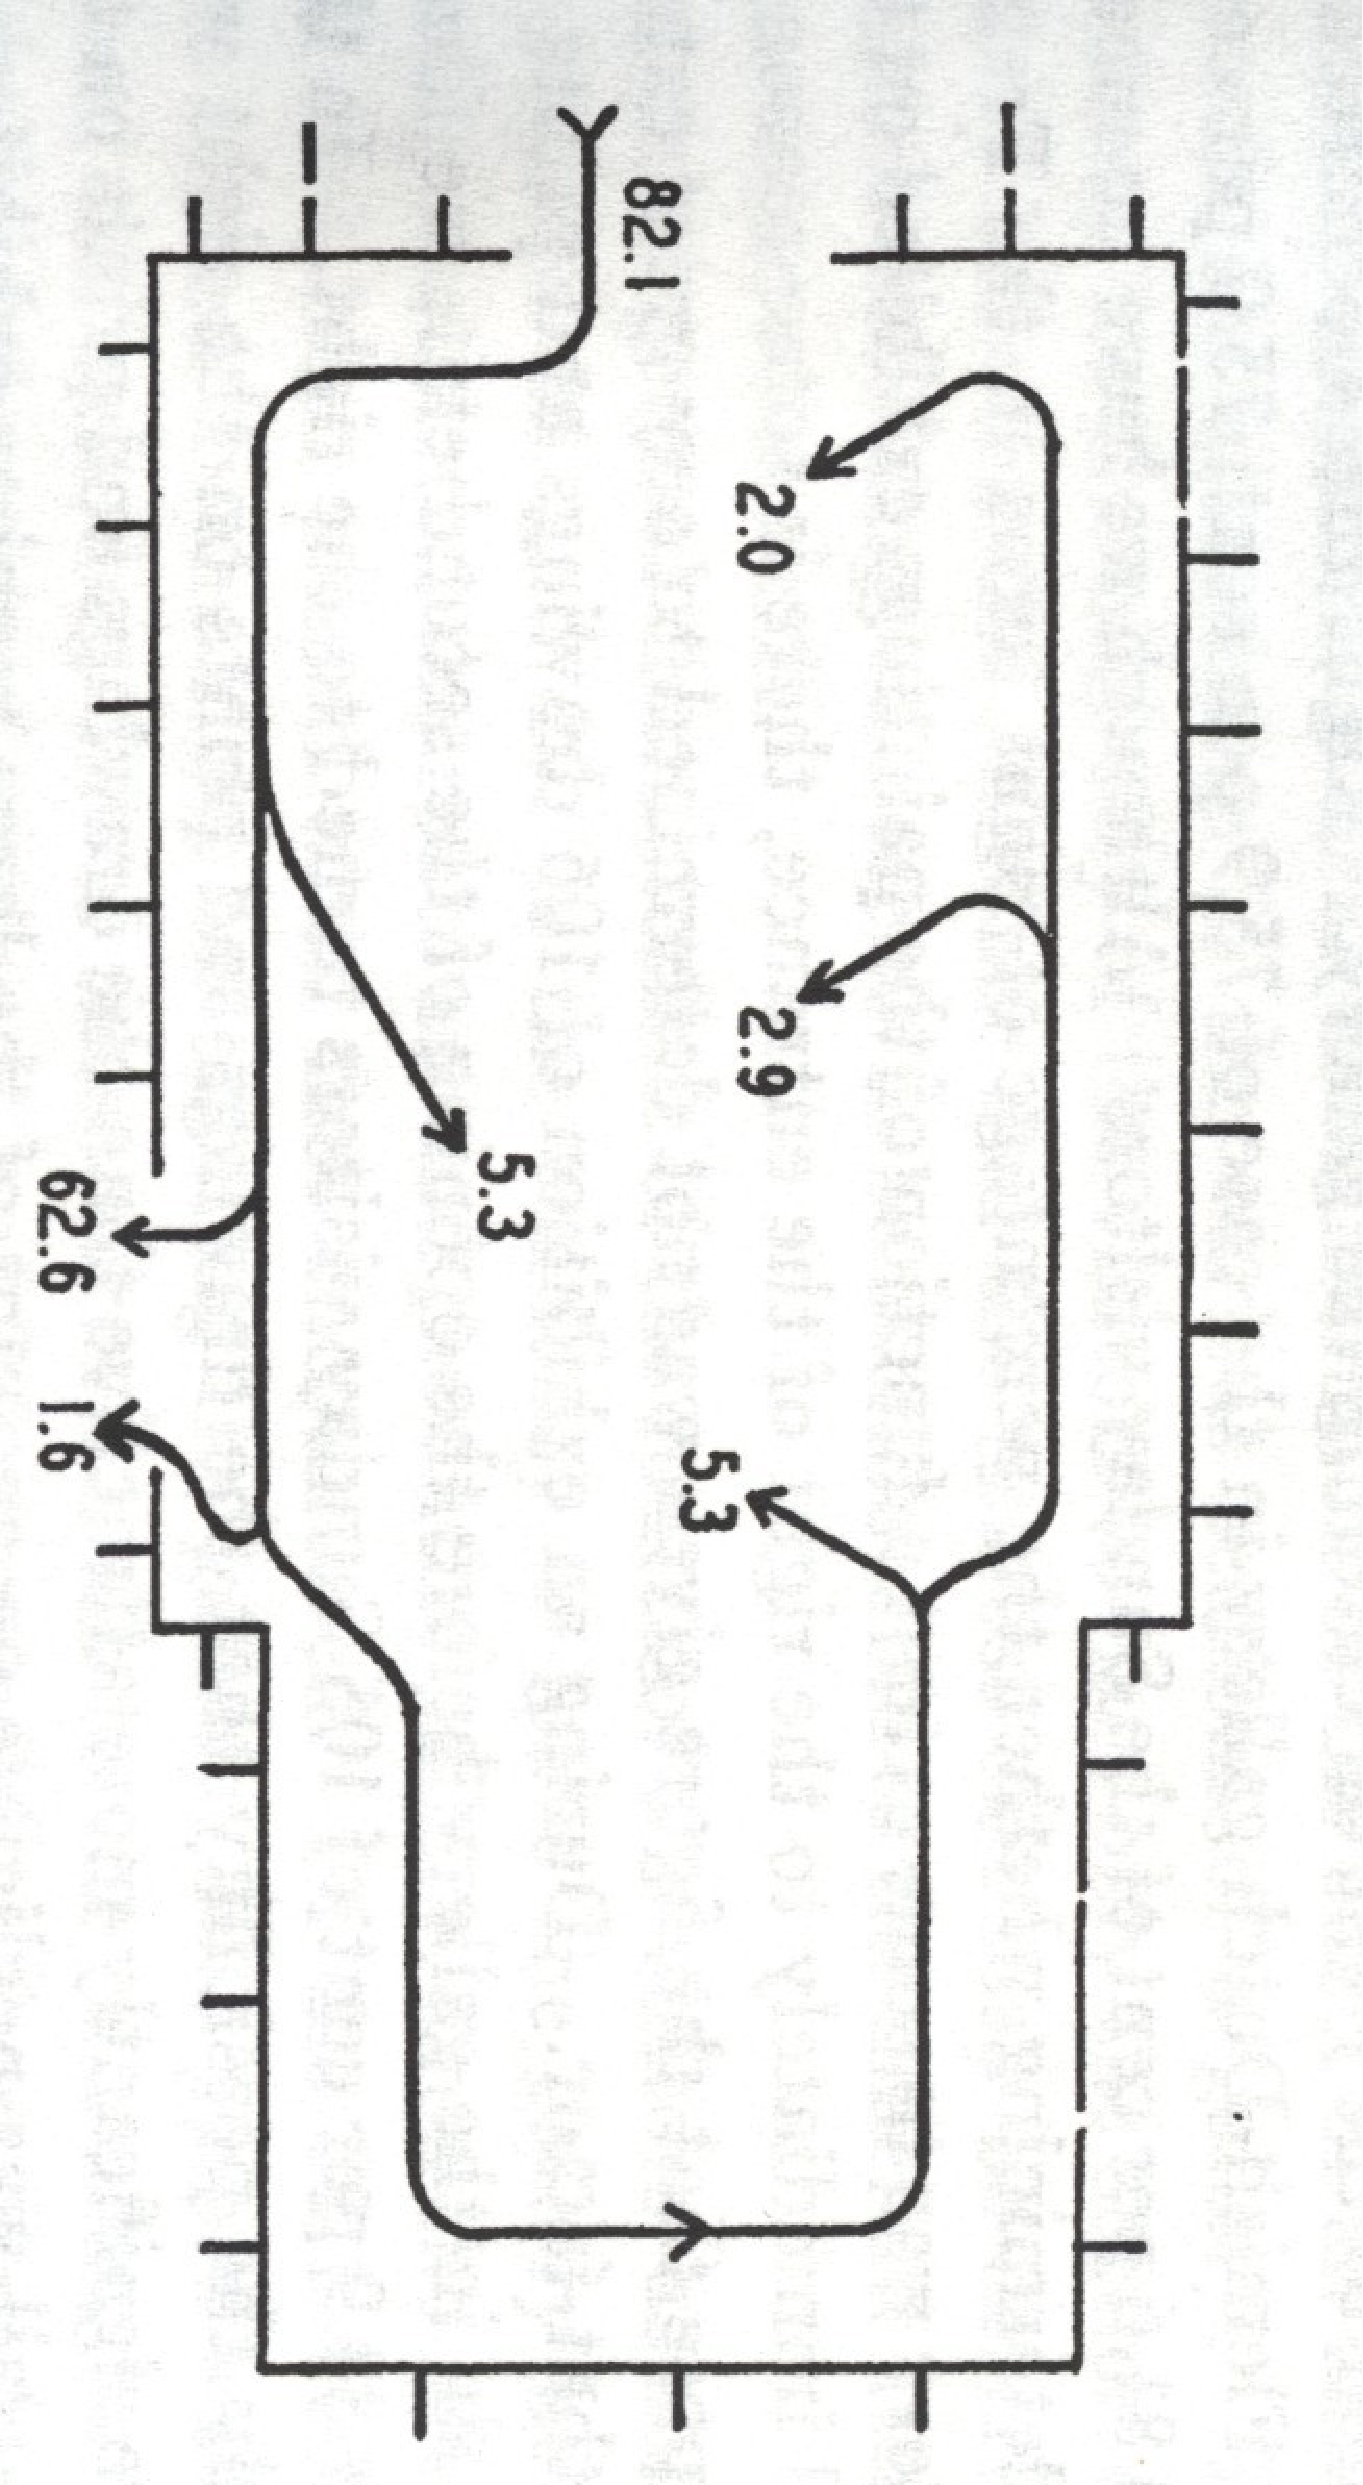
\includegraphics[width=35mm, angle=90]{melton-circulation}}
 \hspace{10 mm}
 \subfloat[frequency of visits]{\label{fig:door-opposite}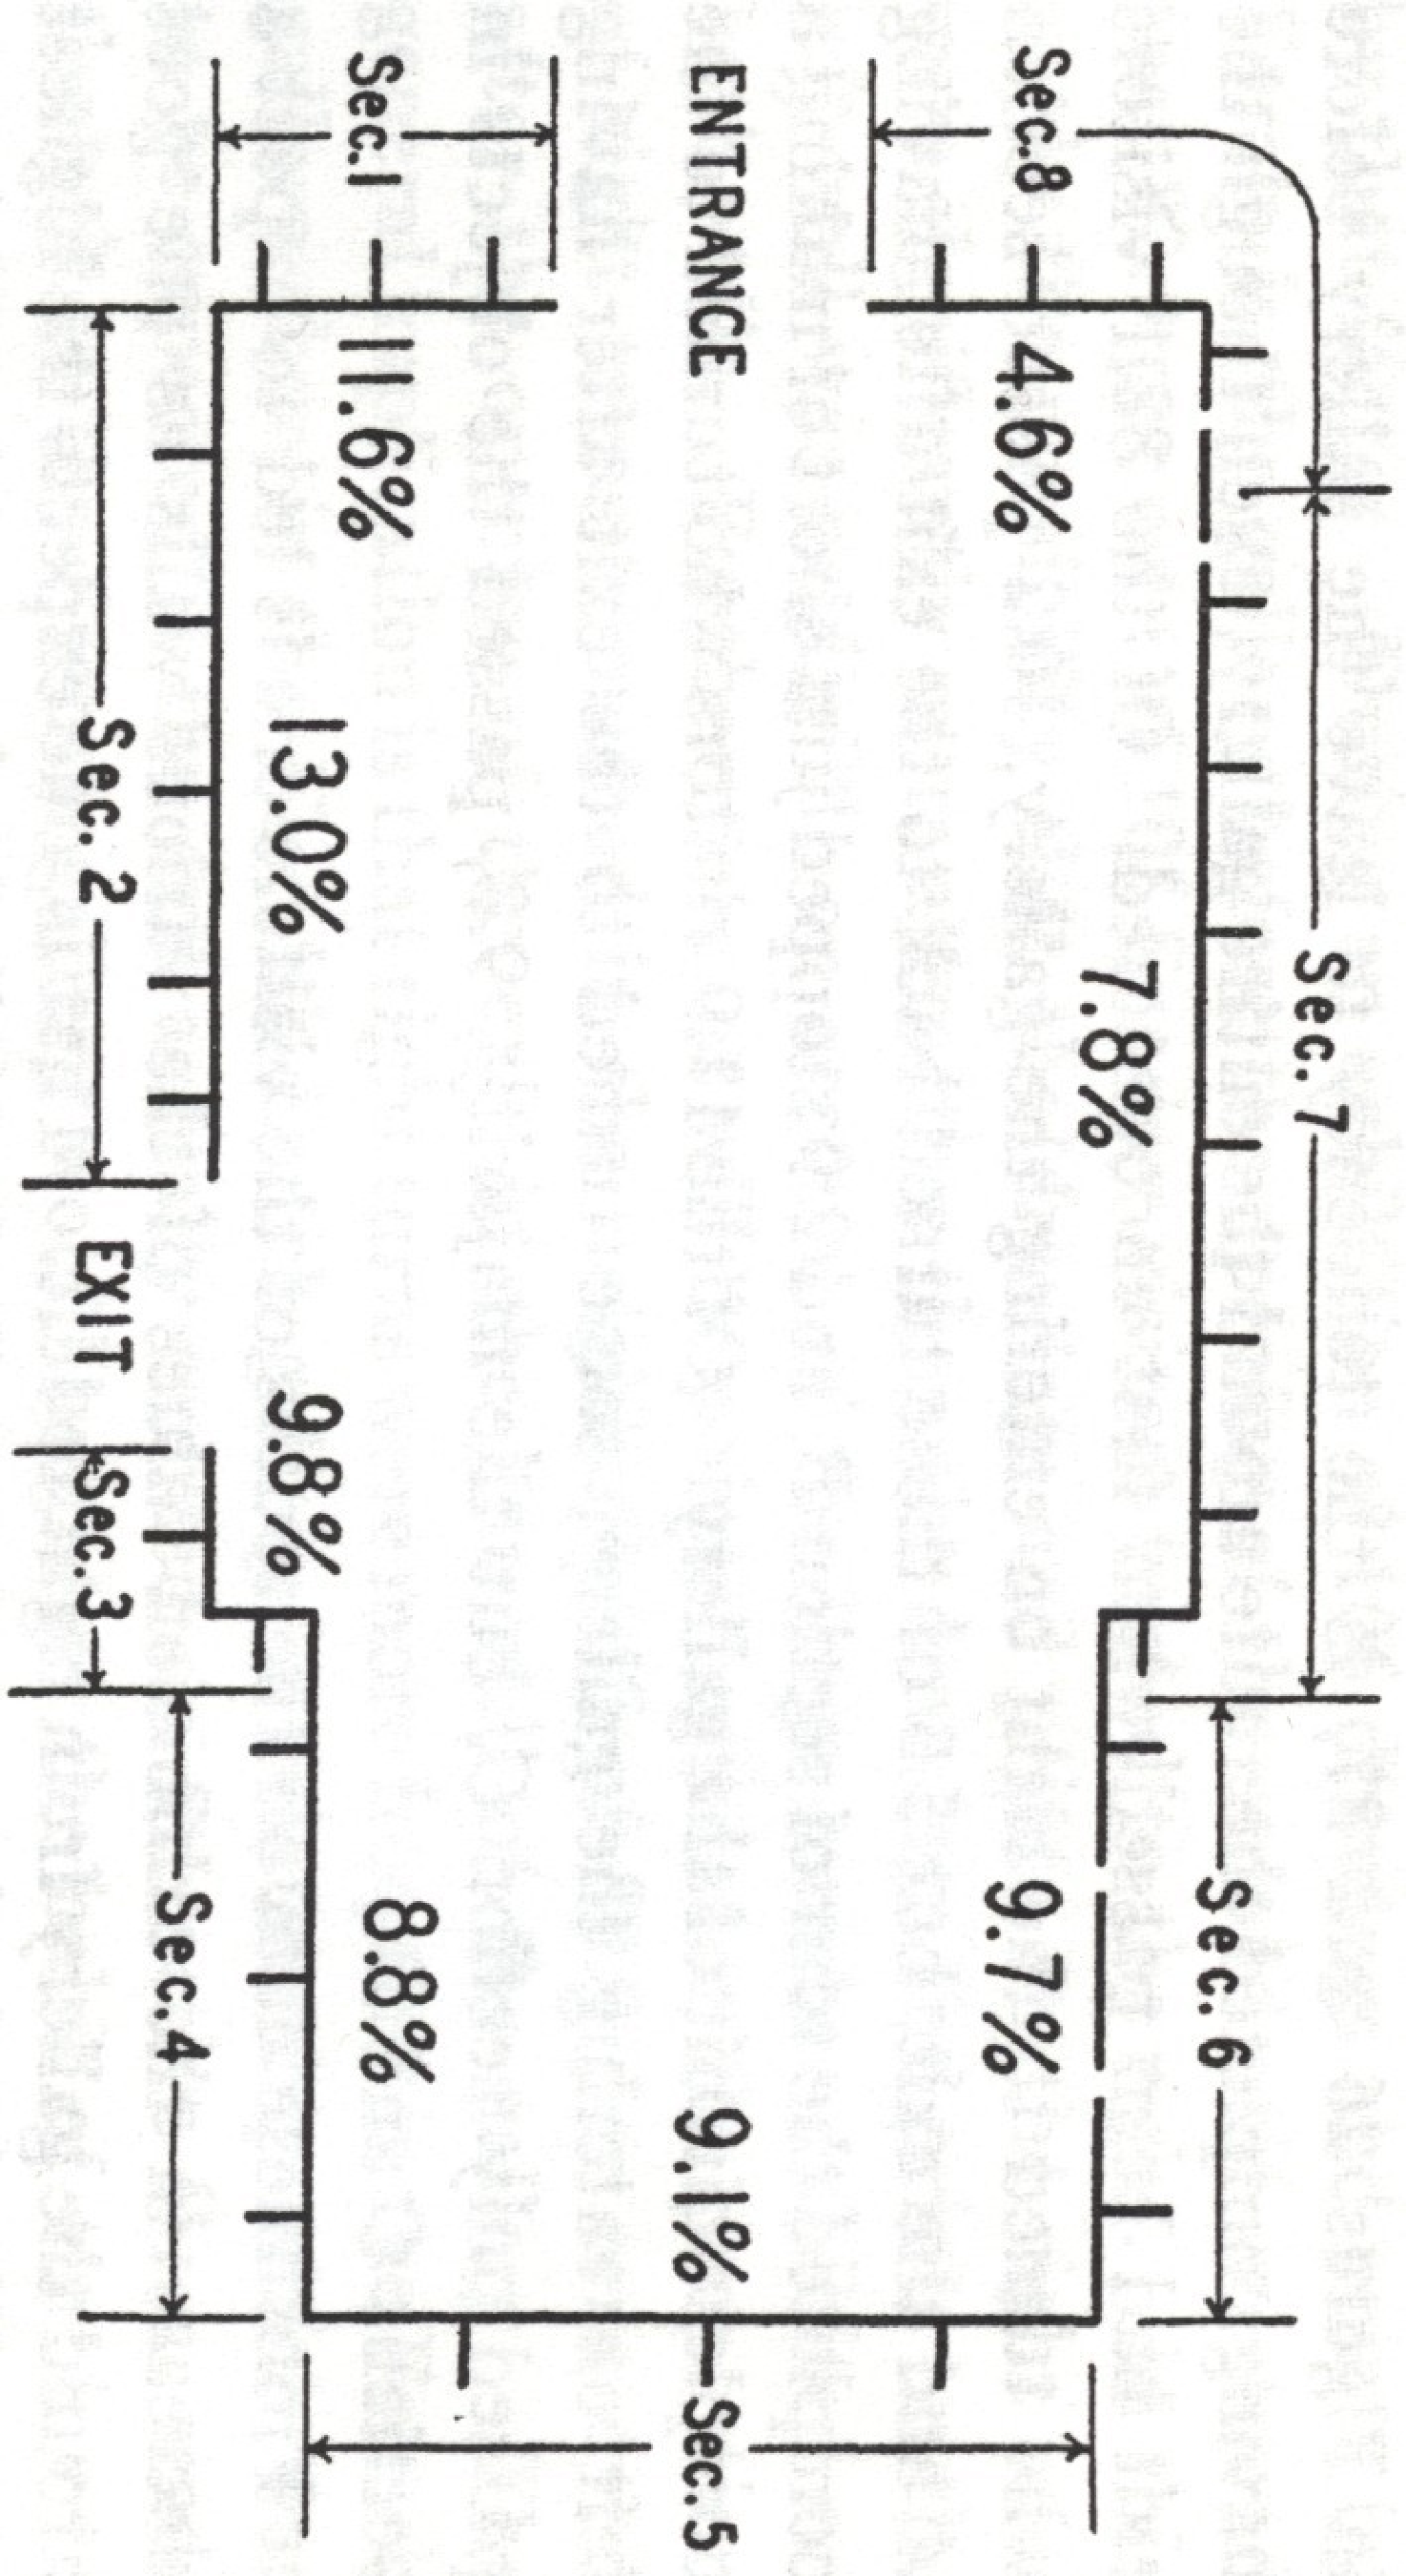
\includegraphics[width=35mm, angle=90]{melton-frequency}}
 \label{melton}
 \caption{Results from Melton's experiments on the effects of door positioning in an Art Museum}
\label{Melton-studies}
\end{figure}

The crux of Melton's experiments suggested that visitors exit through the first door they encounter, which he referred to as the exit gradient. Figure \ref{Melton-studies} shows the results of an extensive study of visitors circulation patterns and stopping frequencies in an art museum. The studies reported that almost 80 percent of visitors exited through the first exit they encountered before viewing the entire exhibition. Additionally, the studied showed that the most frequently visited objects where those located along the shortest path from the entrance to the exit. 

Furthermore, Bitgood suggests that visitors tend to follow along the wall that is closest to the door they entered \cite{Bitgood95}. Given that visitors also tend to exit through the first doorway they encounter, doorways should not be positioned in a wall that is adjacent to an entrance. 

The results of Melton's and Bitgood's studies inform architects of spatial characteristics that influence movement patterns in exhibitions. Specifically, doorways that are positioned on the same side of the room and doorways that are position in a wall adjacent to an entrance cause visitors to pay attention to fewer exhibits than doorways that are positioned on opposing sides of the room and in walls that are not adjacent to entrances.

\begin{description}
\item[Requirement 1:] \emph{Exhibition doorways should be positioned on opposing sides of a gallery room and should not be positioned on a wall that is adjacent to another doorway.} 
\end{description}

Figure \ref{door-position} shows a possible exhibition design where the red door is positioned on the same side of the room as the entrance, while the black door is positioned on the opposing side.
\begin{figure}[H]
\centering
\subfloat[consistent design]{\label{fig:door-opposite}
\includegraphics[width=85mm]{door-possitioning}}
\caption{Schematization of the opposing door requirement.}
\label{door-position}
\end{figure} 


\subsubsection{Spatial arrangement of display cases}
The spatial arrangement of display cases in galleries has been shown to influence visitors' movement patterns. \cite{Bitgood92} showed that display case arrangements that form a perimeter or a peninsula generate the most amount of attention, while display case arrangements that form an island in the middle of the room received the lowest amount of attention.

   \begin{figure}[H]
 \centering
 \subfloat[island]{\label{fig:door-opposite}
\includegraphics[width=35mm]{island}}
 \hspace{10 mm}
 \subfloat[perimeter]{\label{fig:door-opposite}
\includegraphics[width=35mm]{perimeter}}
  \hspace{10 mm}
 \subfloat[peninsula]{\label{fig:door-opposite}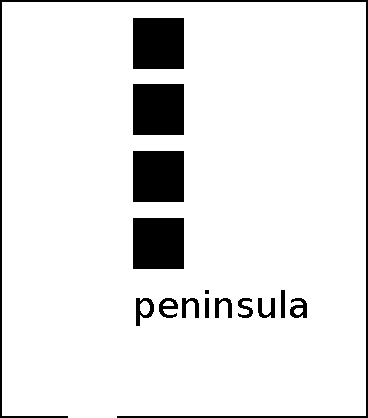
\includegraphics[width=35mm]{peninsula}}
 \caption{Display case arrangements}
\label{display-arrangement}
\end{figure}
 
\begin{description}
\item[Requirement 2:] \emph{Display case arrangements should not form an island near the center of the room.}
\end{description} 

Circulation patterns can be disrupted when a peninsula arrangement cuts horizontally across the view of a visitor as they are entering the room. This type of display pattern will cut off part of the room from the visitor and will make it less likely to be visited.

\begin{description}
\item[Requirement 3:] \emph{Display cases arrangements that form a peninsula should not cut horizontally across the view of a visitor located at an entrance.}
\end{description} 

\begin{figure}[H]
\centering
\subfloat[consistent design]{\label{fig:door-opposite}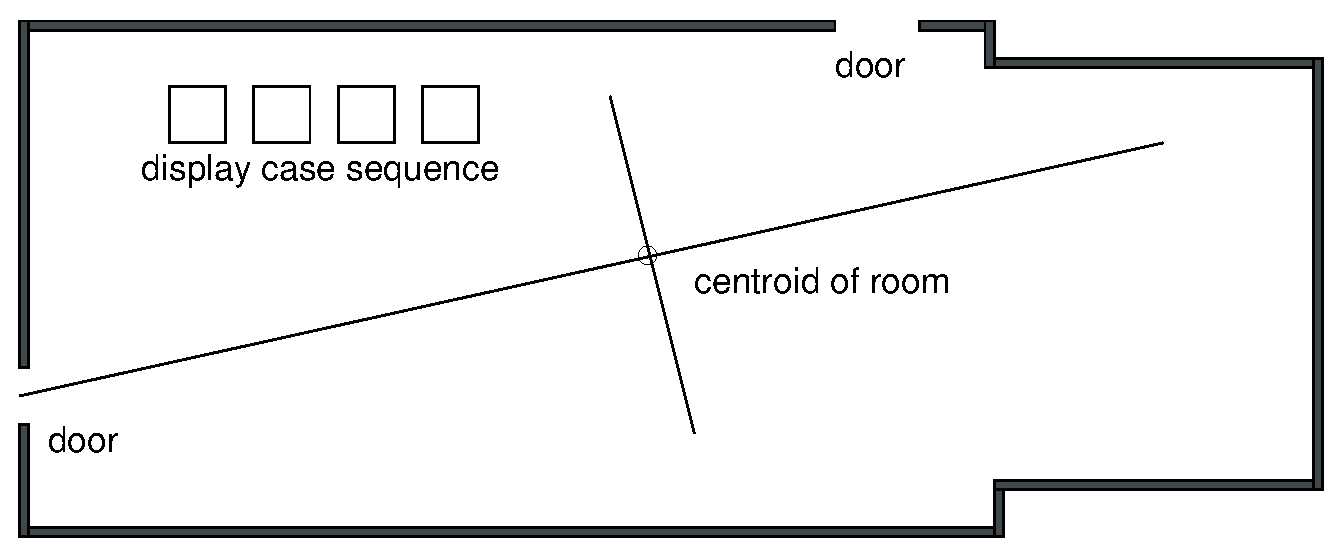
\includegraphics[width=65mm]{display-not-cut}}
\hspace{10 mm}
\subfloat[inconsistent design]{\label{fig:door-opposite}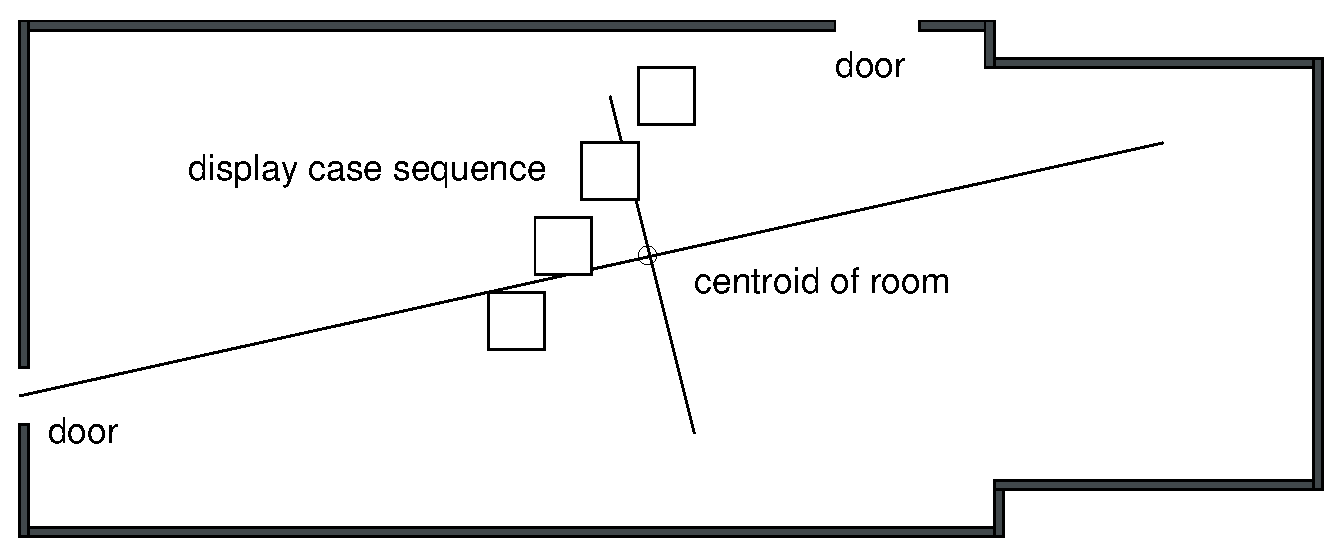
\includegraphics[width=65mm]{door-cut-room}}
\end{figure}


\subsubsection{Congestion}
Congestion in museums can be caused by interference of displayed objects and their viewing spaces with movement pathways of visitors. In order to reduce congestion in museums, designers should be aware of the placement of display cases, statues, furniture (seating benches), and information kiosks within the gallery. The following are requirements that should be followed to reduce congestion in museums:

\begin{description}
\item[Requirement 4:] \emph{There should be no artefactual interference between architectural entities, museum display cases, museum seating, and information kiosks.}
\end{description}

\subsubsection{Positioning of benches, statues, and information kiosks}
The positioning and orientation of benches and statues can increase the amount of attention an exhibition receives and change circulation patterns within a gallery \cite{Stavroulaki} \cite{Museum}. Studies have shown that seating directly facing an object will increase the attention the object receives, even if no one uses the seating. 

\begin{description}
\item[Requirement 5:] \emph{Seating should directly face a gallery wall or display case.}
\end{description}

The orientation of a statue to doorways can increase the attention the statue receives as well as the object close to it. Statues that face away from doorways encourage visitors to move around the statues in order to get a better view.  
\begin{description}
\item[Requirement 6:] \emph{Statues should face away from doorways.}
\end{description}

\subsubsection{Visitor Orientation in the lobby}
The lobby is the first place visitors encounter when they enter a museum. The design of the lobby is important because it not only provides a first glimpse of the museum's exhibits but it is the place where the museum provides services to its visitors, including: a ticketing desk, bathrooms, an information desk, and entrances to exhibitions \cite{Bitgood02}. The aim of the requirements for the lobby focus on making it easy for visitors to locate services and orient themselves to the new environment. 

Upon entering the lobby most visitors need to find the ticket area and/or an information desk. It is important, therefore, that the ticketing area and information desk are visible from the entrance. Additionally, studies have shown that people first look to their right hand side when entering a building. By placing the ticket and information desks on the right hand side of the lobby, visitors are more likely to notice them immediately when they enter the lobby. Finally, the ticketing area should be close to visitors when they enter because it is likely one of the first places they will need to visit.
\begin{description}
\item[Requirement 7:] \emph{The ticketing and information desks should be visible from the main entrance, they should be on the right hand side of the lobby from the main entrance, and they should be on the same side fo the lobby as the  entrance.}
\end{description}

After obtaining a ticket most visitors will be trying to locate the entrance to the exhibitions. Therefore, exhibition entrances should be clearly visible from several parts of the lobby, including the ticketing desk, information desk, and a central lobby location, to make it easy for visitors to find where they need to go. 
\begin{description}
\item[Requirement 8:] \emph{Exhibit entrances should be visible from the ticketing desk, information desk, and a central lobby location.}
\end{description}

Bathrooms are an important services for museum visitors. Surprisingly, the place of the bathroom can have an impact on how long visitors stay in the museum. Studies \cite{tbd} have found that bathrooms that are located on the same side of the lobby as the entrance / exit encourage visitors to leave earlier compared to museums with bathrooms on the opposing side of the lobby from the entrance / exit. Additionally, the doorways to the bathroom should be private to maintain as much privacy in the bathroom as possible.

\begin{description}
\item[Requirement 9:] \emph{The bathroom should be on the opposing side of the lobby from the entrance / exit and the bathroom doorways should be private.}
\end{description}


\subsection{Exploration}
The way visitors explore an exhibition is influenced by the spatial characteristics of the layout, as well as the characteristics of each gallery room. Layouts that are sequential, i.e. one way in / one way out, promote a controlled and orderly flow of movement. Museums of history and science are well served by this type of design because they have a narrative to tell that is chronological. On the other hand, layouts that present the visitor with path choices, i.e. multiple doorways, promote free-flowing exploration. In this type of layout it is important that visitors are aware of the path choices that are available. This means that doorways are visible between each other throughout the layout. This concept of visibility between a network of points is referred to as continuity and is an important characteristic of layouts that present visitors with multiple path choices.  

\begin{description}
\item[Requirement 10:] The layout of the museum should maintain continuity between doorways within each exhibition and gallery room.
\end{description}

Within a Gallery, rooms that are open promote more free-flowing exploration than rooms that are narrow. Narrow rooms inhibit exploration because of space limitations and confinement. Rooms that are open provide more space for visitors to explore the room in a free-flowing manner.
\begin{description}
\item[Requirement 11:] Gallery rooms should be open, rather than confined, in order to promote free-flowing exploration.
\end{description}



\chapter{Case Study: Ranch Style House}


\subsection{A Private Room}
In a particular apartment, the designer wants the bedroom to be private. Given the definition of privacy in this chapter, privacy entails that the bedroom is on the opposing side of the apartment from the main entrance, the bedroom's doorway does not face towards any other doorways, and the doorway is not visible from the main entrance.

Using DSpace, the designer can check for privacy of a bedroom by querying the DSpace representation. The query is a Prolog statement that calls the privacy predicate with the bedroom's unique DSpace identifier. The statement will return true if the bedroom meets the constraint defined by privacy and will return fail if it does not. The floor plans in Figure \ref{room-privacy} show two apartments with a private and un-private bedroom. Given these two floor plans DSpace will validate the floor plan that is private based on the spatial characteristics of the design that define privacy. For example, given Figure \ref{fig:private-room-con} has a unique DSpace identifier of \emph{bedroom1} and Figure \ref{fig:private-room-incon} has a unique DSpace identifier of \emph{bedroom2} the privacy query for bedroom1 will respond with \emph{true} while the query for bedroom2 will respond with \emph{fail}: 
\begin{verbatim}
   ?- privacy(bedroom1).
   true.
   
   ?- privacy(bedroom2).
   fail.
\end{verbatim}

The constraints that define privacy for a room are broken down into three QSAs:
\begin{verbatim}
   opposing(main entrance, bedroom, apartment).
   facing_away(doorway, doorways).
   not_visible(main entrance, doorway).
\end{verbatim}
These three QSA constraints are in turn broken down into qualitative spatial relationships. For example, the opposing side relationship is broken down into SCC relationships for the architectural entities (main entrance, bedroom) point abstractions.
\begin{verbatim}
   SCC1(main entrance, apartment centroid, bedroom).
   SCC2(main entrance, apartment centroid, bedroom).
   SCC3(main entrance, apartment centroid, bedroom).
\end{verbatim}
These SCC relationships are grounded to the quantitative representation via qualification. The SCC constraints are solved for using the orientational constraint solver.

\subsection{Sink / Doorway Artefact Interaction}
In a particular bathroom there is a design requirement that there should be no artefactual interactions between bathroom entities to ensure proper circulation throughout the bathroom. This includes the requirement that the functional space of all sinks should not interfere with the functional space of a doorway. 

TODO: figure for two bathrooms

Using DSpace a designer can check that there are no artefactual interactions by querying the design representation. The query is a Prolog statement that check for the topological structures of the bathrooms artefactual extension. For example, Figure \ref{?} shows two example bathroom floor plans. Figure \ref{?} shows a bathroom design that is consisted per the requirement and Figure \ref{?} shows a bathroom design that is inconsistent per the requirement. Given these two designs and ids for the sink (\emph{sink55}), and door (\emph{door104}), the following query can be made to check for artefactual interaction:
\begin{verbatim}
   artefactual_interaction(sink55, door104).
\end{verbatim}
The query will return \emph{true} for Figure \ref{?} and will fail for Figure \ref{?}.

The $artefactual\_interaction$ predicate is broken down into topological constraints that check for partially overlapping topological relationships between the artefactual extensions of the bathroom doorway and sink. The topological constraints are solved in the topological constraint solver. 




\chapter{Evaluation}


\chapter{Future Work / Conclusion}

\appendix
\chapter{Appendix}
\section{Spatial Abstraction of Architectural Entities}
The remainder of this section shows how architectural entities and interior designs objects are spatially abstracted into points, directed points, and convex hulls and how they are transformed in DSpace. Table \ref{spatial abstractions} shows which spatial abstractions each architectural entity can be transformed into. 

\begin{table}[H]
  \begin{center}
  \begin{tabular}{ | r | c | c | c |}
    \hline
    entity & point & directed point & convex hull\\ \hline
    doorway & X & X & X \\ \hline
    window & X & X & X \\ \hline
    wall & X & X & X \\ \hline
    column & X &  & X \\ \hline
    space & X &  & X \\ \hline
    interior design object & X & X* & X \\
    \hline
  \end{tabular}
  \end{center}
\caption{Spatial Abstractions for Architectural Entities}
\label{spatial abstractions}
\end{table} 

\noindent \emph{\large Point} \\
\indent All architectural entities and interior design objects have a point abstraction that is defined as the centroid of the entity's physical polygon space. Figure \ref{point-abs} shows the point abstraction for a doorway. Note that the point is the centroid of the doorway's physical geometry. The point abstraction is used in orientational reasoning and is therefore used as an approximation of the object's location in the design. In general, the centroid is a good point approximation of location because it is a generalization of polygon space as a single point. 
\begin{verbatim}
   point_abstraction(door1, Point) :-
           quantitative_geometry(door1, Quant),
           centroid(Quant, Point).
\end{verbatim}

\begin{figure}[H]
\centering
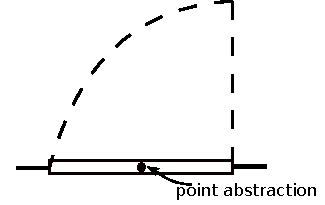
\includegraphics[width=70mm]{point-abs}
\caption{Doorway Point Abstraction}
\label{point-abs}
\end{figure}

\noindent \emph{\large Directed Point} \\
\indent Walls, doorways, windows, and some interior design objects have a directed point abstraction. A directed point is represented as a tuple (\emph{Cartesian point}, \emph{direction}). The point is defined as the centroid of the quantitative polygon space, as it is in the point abstraction. The direction is defined either by the user, as is the case for interior design objects, or by an intrinsic spatial property of the entity, as is the case for doorways, walls, and windows.

For these entities, direction is based on the interpretation of the nature of the entity within the context of a design. Formally, direction is interpreted as a vector that emanates from an entity's point abstraction towards the room / space it is contained in. Specifically, direction is defined as the perpendicular vector to the intrinsic x-axis of the object. Figure \ref{dir-point-abs} shows the directed point abstraction for a doorway. Not that the direction is perpendicular to the x-axis of the doorway's physical geometry. Based on this definition there will be two perpendicular lines that define the direction. In this situation, the context of the space in which the entity is located is need to decided which of the two directions to use.  

\begin{verbatim}
   dir_point_abstraction(door1, (Point, Dir), room3) :-
           quantitative_geometry(door1, Quant),
           centroid(Quant, Point),
           direction(Quant, Point, room3, Dir).
\end{verbatim}

\begin{figure}[H]\label{dir-point-abs}
\centering

\includegraphics[width=70mm]{dir-point-abs}
\caption{Doorway Point Abstraction}
\end{figure}

\noindent \emph{\large Convex Hull} \\
\indent All architectural entities have a convex hull abstraction. The convex hull is calculated over the quantitative polygon space by using the divide and conquer convex hull algorithm \cite{tbd}. The result of the algorithm is a convex hull representation that is a list of points sorted in counterclockwise order. Convex hulls are used in topological reasoning.
\begin{verbatim}
   convex_hull_abstraction(door1, ConvexHull).
           quantitative_geometry(door1, Quant),
           convex_hull(convex, ConvexHull).
\end{verbatim}

TODO: figure for convex hull abs

% ------------- End main chapters ----------------------

\clearpage
\bibliographystyle{abbrv}
\bibliography{museum}
%\bibliography{architecture}
\bibliography{qsr}
%\bibliography{clp}
%\bibliography{relatedworks}

%\addcontentsline{toc}{chapter}{Bibliography}

\end{document}
